\documentclass[1p]{elsarticle_modified}
%\bibliographystyle{elsarticle-num}

%\usepackage[colorlinks]{hyperref}
%\usepackage{abbrmath_seonhwa} %\Abb, \Ascr, \Acal ,\Abf, \Afrak
\usepackage{amsfonts}
\usepackage{amssymb}
\usepackage{amsmath}
\usepackage{amsthm}
\usepackage{scalefnt}
\usepackage{amsbsy}
\usepackage{kotex}
\usepackage{caption}
\usepackage{subfig}
\usepackage{color}
\usepackage{graphicx}
\usepackage{xcolor} %% white, black, red, green, blue, cyan, magenta, yellow
\usepackage{float}
\usepackage{setspace}
\usepackage{hyperref}

\usepackage{tikz}
\usetikzlibrary{arrows}

\usepackage{multirow}
\usepackage{array} % fixed length table
\usepackage{hhline}

%%%%%%%%%%%%%%%%%%%%%
\makeatletter
\renewcommand*\env@matrix[1][\arraystretch]{%
	\edef\arraystretch{#1}%
	\hskip -\arraycolsep
	\let\@ifnextchar\new@ifnextchar
	\array{*\c@MaxMatrixCols c}}
\makeatother %https://tex.stackexchange.com/questions/14071/how-can-i-increase-the-line-spacing-in-a-matrix
%%%%%%%%%%%%%%%

\usepackage[normalem]{ulem}

\newcommand{\msout}[1]{\ifmmode\text{\sout{\ensuremath{#1}}}\else\sout{#1}\fi}
%SOURCE: \msout is \stkout macro in https://tex.stackexchange.com/questions/20609/strikeout-in-math-mode

\newcommand{\cancel}[1]{
	\ifmmode
	{\color{red}\msout{#1}}
	\else
	{\color{red}\sout{#1}}
	\fi
}

\newcommand{\add}[1]{
	{\color{blue}\uwave{#1}}
}

\newcommand{\replace}[2]{
	\ifmmode
	{\color{red}\msout{#1}}{\color{blue}\uwave{#2}}
	\else
	{\color{red}\sout{#1}}{\color{blue}\uwave{#2}}
	\fi
}

\newcommand{\Sol}{\mathcal{S}} %segment
\newcommand{\D}{D} %diagram
\newcommand{\A}{\mathcal{A}} %arc


%%%%%%%%%%%%%%%%%%%%%%%%%%%%%5 test

\def\sl{\operatorname{\textup{SL}}(2,\Cbb)}
\def\psl{\operatorname{\textup{PSL}}(2,\Cbb)}
\def\quan{\mkern 1mu \triangleright \mkern 1mu}

\theoremstyle{definition}
\newtheorem{thm}{Theorem}[section]
\newtheorem{prop}[thm]{Proposition}
\newtheorem{lem}[thm]{Lemma}
\newtheorem{ques}[thm]{Question}
\newtheorem{cor}[thm]{Corollary}
\newtheorem{defn}[thm]{Definition}
\newtheorem{exam}[thm]{Example}
\newtheorem{rmk}[thm]{Remark}
\newtheorem{alg}[thm]{Algorithm}

\newcommand{\I}{\sqrt{-1}}
\begin{document}

%\begin{frontmatter}
%
%\title{Boundary parabolic representations of knots up to 8 crossings}
%
%%% Group authors per affiliation:
%\author{Yunhi Cho} 
%\address{Department of Mathematics, University of Seoul, Seoul, Korea}
%\ead{yhcho@uos.ac.kr}
%
%
%\author{Seonhwa Kim} %\fnref{s_kim}}
%\address{Center for Geometry and Physics, Institute for Basic Science, Pohang, 37673, Korea}
%\ead{ryeona17@ibs.re.kr}
%
%\author{Hyuk Kim}
%\address{Department of Mathematical Sciences, Seoul National University, Seoul 08826, Korea}
%\ead{hyukkim@snu.ac.kr}
%
%\author{Seokbeom Yoon}
%\address{Department of Mathematical Sciences, Seoul National University, Seoul, 08826,  Korea}
%\ead{sbyoon15@snu.ac.kr}
%
%\begin{abstract}
%We find all boundary parabolic representation of knots up to 8 crossings.
%
%\end{abstract}
%\begin{keyword}
%    \MSC[2010] 57M25 
%\end{keyword}
%
%\end{frontmatter}

%\linenumbers
%\tableofcontents
%
\newcommand\colored[1]{\textcolor{white}{\rule[-0.35ex]{0.8em}{1.4ex}}\kern-0.8em\color{red} #1}%
%\newcommand\colored[1]{\textcolor{white}{ #1}\kern-2.17ex	\textcolor{white}{ #1}\kern-1.81ex	\textcolor{white}{ #1}\kern-2.15ex\color{red}#1	}

{\Large $\underline{12a_{0710}~(K12a_{0710})}$}

\setlength{\tabcolsep}{10pt}
\renewcommand{\arraystretch}{1.6}
\vspace{1cm}\begin{tabular}{m{100pt}>{\centering\arraybackslash}m{274pt}}
\multirow{5}{120pt}{
	\centering
	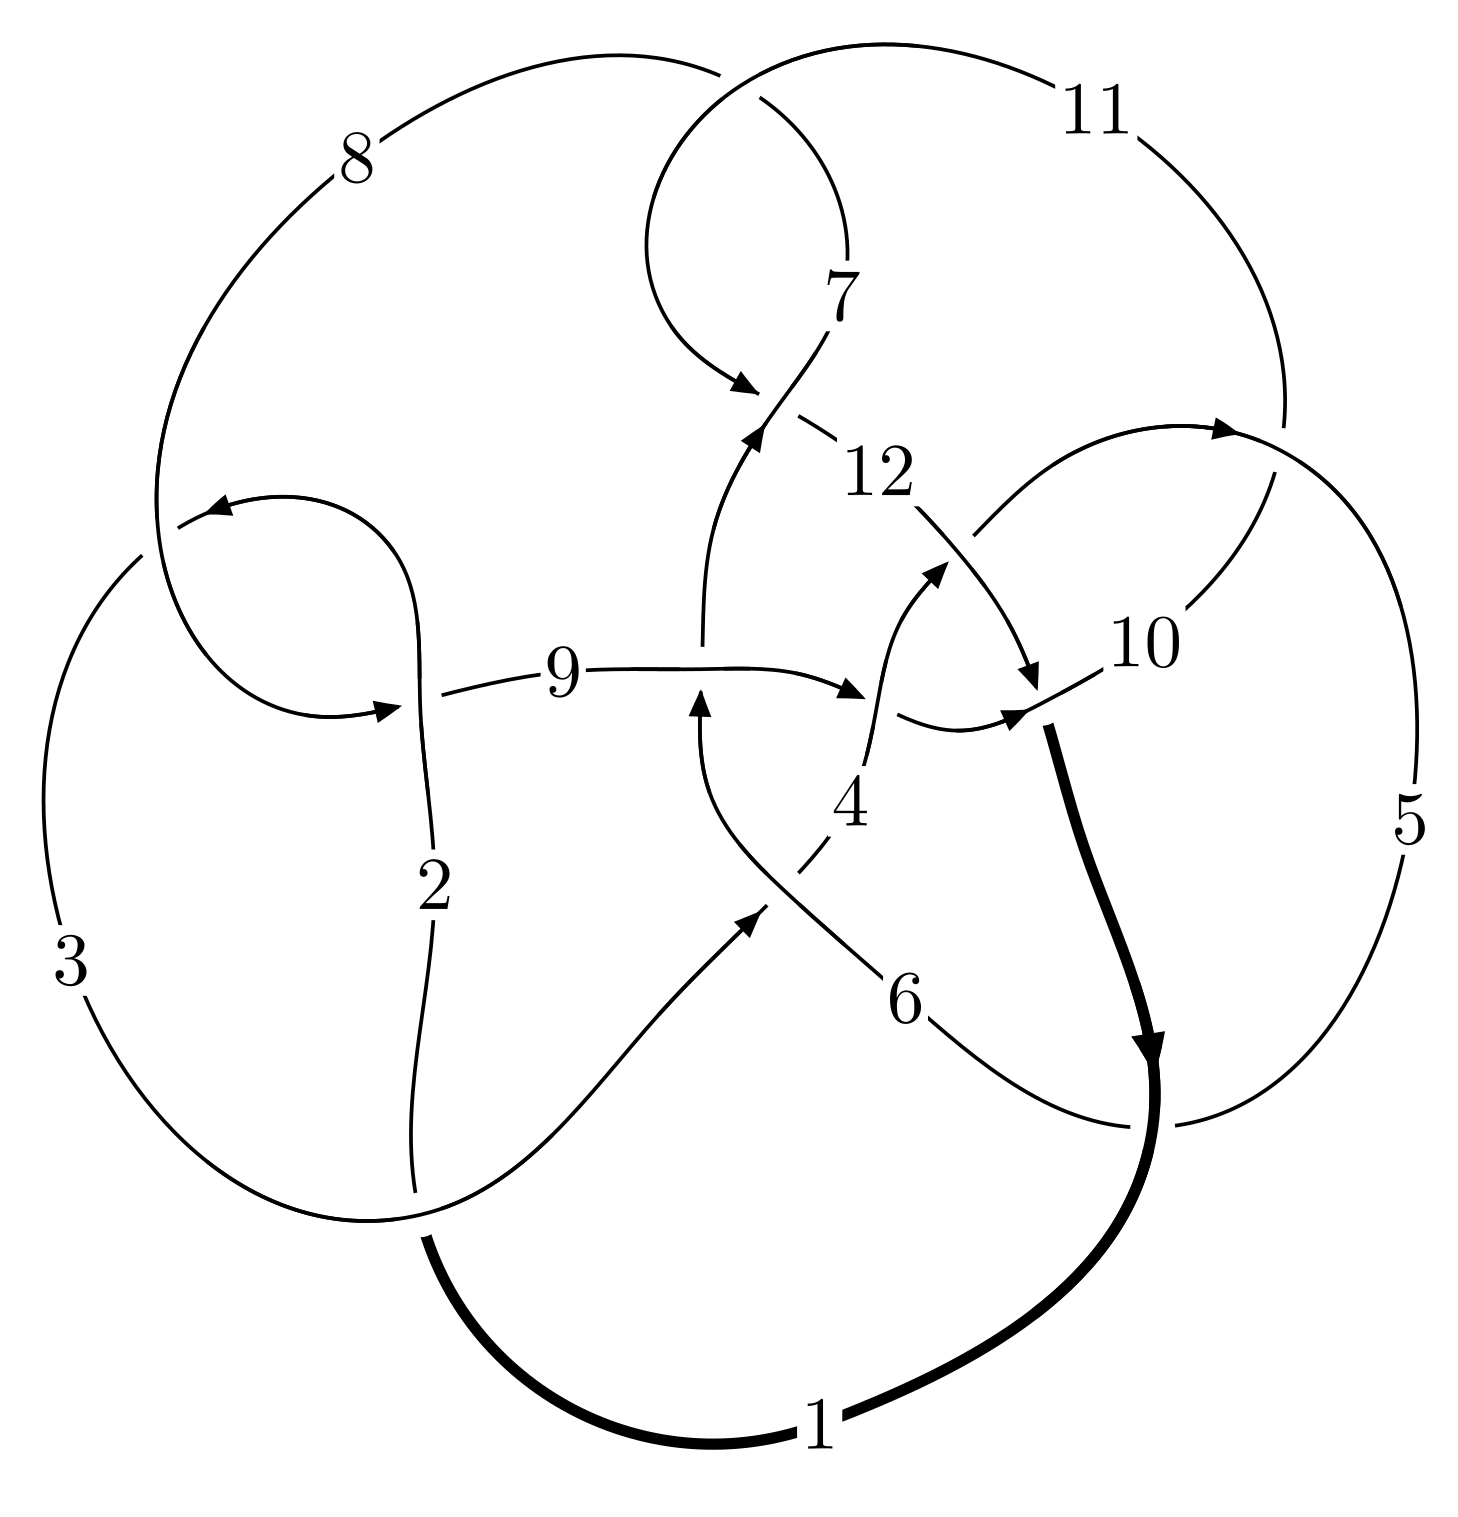
\includegraphics[width=112pt]{../../../GIT/diagram.site/Diagrams/png/1511_12a_0710.png}\\
\ \ \ A knot diagram\footnotemark}&
\allowdisplaybreaks
\textbf{Linearized knot diagam} \\
\cline{2-2}
 &
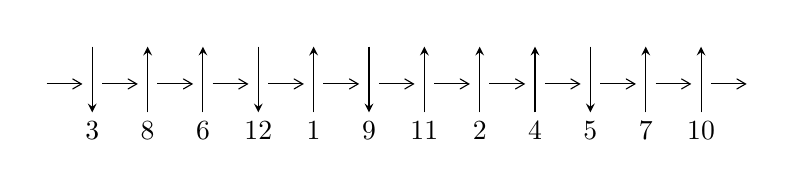
\begin{tikzpicture}[x=20pt, y=17pt]
	% nodes
	\node (C0) at (0, 0) {};
	\node (C1) at (1, 0) {};
	\node (C1U) at (1, +1) {};
	\node (C1D) at (1, -1) {3};

	\node (C2) at (2, 0) {};
	\node (C2U) at (2, +1) {};
	\node (C2D) at (2, -1) {8};

	\node (C3) at (3, 0) {};
	\node (C3U) at (3, +1) {};
	\node (C3D) at (3, -1) {6};

	\node (C4) at (4, 0) {};
	\node (C4U) at (4, +1) {};
	\node (C4D) at (4, -1) {12};

	\node (C5) at (5, 0) {};
	\node (C5U) at (5, +1) {};
	\node (C5D) at (5, -1) {1};

	\node (C6) at (6, 0) {};
	\node (C6U) at (6, +1) {};
	\node (C6D) at (6, -1) {9};

	\node (C7) at (7, 0) {};
	\node (C7U) at (7, +1) {};
	\node (C7D) at (7, -1) {11};

	\node (C8) at (8, 0) {};
	\node (C8U) at (8, +1) {};
	\node (C8D) at (8, -1) {2};

	\node (C9) at (9, 0) {};
	\node (C9U) at (9, +1) {};
	\node (C9D) at (9, -1) {4};

	\node (C10) at (10, 0) {};
	\node (C10U) at (10, +1) {};
	\node (C10D) at (10, -1) {5};

	\node (C11) at (11, 0) {};
	\node (C11U) at (11, +1) {};
	\node (C11D) at (11, -1) {7};

	\node (C12) at (12, 0) {};
	\node (C12U) at (12, +1) {};
	\node (C12D) at (12, -1) {10};
	\node (C13) at (13, 0) {};

	% arrows
	\draw[->,>={angle 60}]
	(C0) edge (C1) (C1) edge (C2) (C2) edge (C3) (C3) edge (C4) (C4) edge (C5) (C5) edge (C6) (C6) edge (C7) (C7) edge (C8) (C8) edge (C9) (C9) edge (C10) (C10) edge (C11) (C11) edge (C12) (C12) edge (C13) ;	\draw[->,>=stealth]
	(C1U) edge (C1D) (C2D) edge (C2U) (C3D) edge (C3U) (C4U) edge (C4D) (C5D) edge (C5U) (C6U) edge (C6D) (C7D) edge (C7U) (C8D) edge (C8U) (C9D) edge (C9U) (C10U) edge (C10D) (C11D) edge (C11U) (C12D) edge (C12U) ;
	\end{tikzpicture} \\
\hhline{~~} \\& 
\textbf{Solving Sequence} \\ \cline{2-2} 
 &
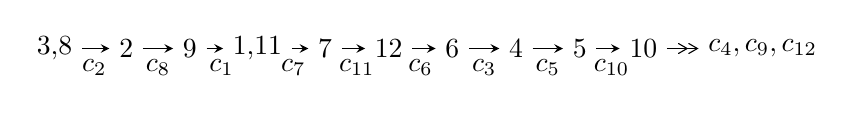
\begin{tikzpicture}[x=23pt, y=7pt]
	% node
	\node (A0) at (-1/8, 0) {3,8};
	\node (A1) at (1, 0) {2};
	\node (A2) at (2, 0) {9};
	\node (A3) at (49/16, 0) {1,11};
	\node (A4) at (33/8, 0) {7};
	\node (A5) at (41/8, 0) {12};
	\node (A6) at (49/8, 0) {6};
	\node (A7) at (57/8, 0) {4};
	\node (A8) at (65/8, 0) {5};
	\node (A9) at (73/8, 0) {10};
	\node (C1) at (1/2, -1) {$c_{2}$};
	\node (C2) at (3/2, -1) {$c_{8}$};
	\node (C3) at (5/2, -1) {$c_{1}$};
	\node (C4) at (29/8, -1) {$c_{7}$};
	\node (C5) at (37/8, -1) {$c_{11}$};
	\node (C6) at (45/8, -1) {$c_{6}$};
	\node (C7) at (53/8, -1) {$c_{3}$};
	\node (C8) at (61/8, -1) {$c_{5}$};
	\node (C9) at (69/8, -1) {$c_{10}$};
	\node (A10) at (11, 0) {$c_{4},c_{9},c_{12}$};

	% edge
	\draw[->,>=stealth]	
	(A0) edge (A1) (A1) edge (A2) (A2) edge (A3) (A3) edge (A4) (A4) edge (A5) (A5) edge (A6) (A6) edge (A7) (A7) edge (A8) (A8) edge (A9) ;
	\draw[->>,>={angle 60}]	
	(A9) edge (A10);
\end{tikzpicture} \\ 

\end{tabular} \\

\footnotetext{
The image of knot diagram is generated by the software ``\textbf{Draw programme}" developed by Andrew Bartholomew(\url{http://www.layer8.co.uk/maths/draw/index.htm\#Running-draw}), where we modified some parts for our purpose(\url{https://github.com/CATsTAILs/LinksPainter}).
}\phantom \\ \newline 
\centering \textbf{Ideals for irreducible components\footnotemark of $X_{\text{par}}$} 
 
\begin{align*}
I^u_{1}&=\langle 
2.03244\times10^{803} u^{198}-3.73750\times10^{803} u^{197}+\cdots+2.91199\times10^{803} b-7.79066\times10^{806},\\
\phantom{I^u_{1}}&\phantom{= \langle  }5.88369\times10^{805} u^{198}-4.46985\times10^{805} u^{197}+\cdots+1.45396\times10^{807} a-2.49046\times10^{808},\\
\phantom{I^u_{1}}&\phantom{= \langle  }u^{199}-2 u^{198}+\cdots+2292 u+4993\rangle \\
I^u_{2}&=\langle 
-4.40584\times10^{28} u^{49}+2.00303\times10^{29} u^{48}+\cdots+4.27060\times10^{28} b+7.48072\times10^{28},\\
\phantom{I^u_{2}}&\phantom{= \langle  }1.07238\times10^{28} u^{49}-2.47638\times10^{28} u^{48}+\cdots+4.27060\times10^{28} a-1.90703\times10^{28},\;u^{50}-3 u^{49}+\cdots-5 u+1\rangle \\
\\
\end{align*}
\raggedright * 2 irreducible components of $\dim_{\mathbb{C}}=0$, with total 249 representations.\\
\footnotetext{All coefficients of polynomials are rational numbers. But the coefficients are sometimes approximated in decimal forms when there is not enough margin.}
\newpage
\renewcommand{\arraystretch}{1}
\centering \section*{I. $I^u_{1}= \langle 2.03\times10^{803} u^{198}-3.74\times10^{803} u^{197}+\cdots+2.91\times10^{803} b-7.79\times10^{806},\;5.88\times10^{805} u^{198}-4.47\times10^{805} u^{197}+\cdots+1.45\times10^{807} a-2.49\times10^{808},\;u^{199}-2 u^{198}+\cdots+2292 u+4993 \rangle$}
\flushleft \textbf{(i) Arc colorings}\\
\begin{tabular}{m{7pt} m{180pt} m{7pt} m{180pt} }
\flushright $a_{3}=$&$\begin{pmatrix}1\\0\end{pmatrix}$ \\
\flushright $a_{8}=$&$\begin{pmatrix}0\\u\end{pmatrix}$ \\
\flushright $a_{2}=$&$\begin{pmatrix}1\\u^2\end{pmatrix}$ \\
\flushright $a_{9}=$&$\begin{pmatrix}u\\u^3+u\end{pmatrix}$ \\
\flushright $a_{1}=$&$\begin{pmatrix}u^2+1\\u^2\end{pmatrix}$ \\
\flushright $a_{11}=$&$\begin{pmatrix}-0.0404668 u^{198}+0.0307427 u^{197}+\cdots-390.332 u+17.1288\\-0.697956 u^{198}+1.28349 u^{197}+\cdots+923.373 u+2675.37\end{pmatrix}$ \\
\flushright $a_{7}=$&$\begin{pmatrix}0.223072 u^{198}-0.613083 u^{197}+\cdots-569.312 u-1221.06\\0.232181 u^{198}-0.752237 u^{197}+\cdots-3069.01 u-2189.90\end{pmatrix}$ \\
\flushright $a_{12}=$&$\begin{pmatrix}0.172321 u^{198}-0.596347 u^{197}+\cdots-840.099 u-1519.71\\-0.187797 u^{198}+0.0761186 u^{197}+\cdots-408.248 u+798.875\end{pmatrix}$ \\
\flushright $a_{6}=$&$\begin{pmatrix}-0.0469788 u^{198}-0.343566 u^{197}+\cdots-1400.00 u-910.198\\-0.0305804 u^{198}-0.248436 u^{197}+\cdots-1931.16 u-528.014\end{pmatrix}$ \\
\flushright $a_{4}=$&$\begin{pmatrix}0.220317 u^{198}-0.475003 u^{197}+\cdots-694.057 u-673.435\\-0.120181 u^{198}+0.109173 u^{197}+\cdots-1668.53 u-117.751\end{pmatrix}$ \\
\flushright $a_{5}=$&$\begin{pmatrix}0.296790 u^{198}-0.741474 u^{197}+\cdots-573.786 u-1612.16\\0.188571 u^{198}-0.771376 u^{197}+\cdots-3411.19 u-2396.72\end{pmatrix}$ \\
\flushright $a_{10}=$&$\begin{pmatrix}0.205050 u^{198}-0.599328 u^{197}+\cdots-241.616 u-1720.11\\0.0571877 u^{198}-0.344279 u^{197}+\cdots+108.054 u+287.925\end{pmatrix}$\\&\end{tabular}
\flushleft \textbf{(ii) Obstruction class $= -1$}\\~\\
\flushleft \textbf{(iii) Cusp Shapes $= 0.329770 u^{198}+0.827580 u^{197}+\cdots+3619.10 u+1349.38$}\\~\\
\newpage\renewcommand{\arraystretch}{1}
\flushleft \textbf{(iv) u-Polynomials at the component}\newline \\
\begin{tabular}{m{50pt}|m{274pt}}
Crossings & \hspace{64pt}u-Polynomials at each crossing \\
\hline $$\begin{aligned}c_{1}\end{aligned}$$&$\begin{aligned}
&u^{199}+88 u^{198}+\cdots-898659484 u-24930049
\end{aligned}$\\
\hline $$\begin{aligned}c_{2},c_{8}\end{aligned}$$&$\begin{aligned}
&u^{199}+2 u^{198}+\cdots+2292 u-4993
\end{aligned}$\\
\hline $$\begin{aligned}c_{3}\end{aligned}$$&$\begin{aligned}
&16(16 u^{199}-404 u^{198}+\cdots+3748743 u-588397)
\end{aligned}$\\
\hline $$\begin{aligned}c_{4}\end{aligned}$$&$\begin{aligned}
&4(4 u^{199}+34 u^{198}+\cdots+1315 u-115)
\end{aligned}$\\
\hline $$\begin{aligned}c_{5}\end{aligned}$$&$\begin{aligned}
&u^{199}+3 u^{198}+\cdots+150597109870 u-13651828868
\end{aligned}$\\
\hline $$\begin{aligned}c_{6}\end{aligned}$$&$\begin{aligned}
&u^{199}-3 u^{198}+\cdots+22334708 u-1049936
\end{aligned}$\\
\hline $$\begin{aligned}c_{7},c_{11}\end{aligned}$$&$\begin{aligned}
&4(4 u^{199}+6 u^{198}+\cdots- u-1)
\end{aligned}$\\
\hline $$\begin{aligned}c_{9}\end{aligned}$$&$\begin{aligned}
&u^{199}+2 u^{198}+\cdots+15945814 u-22455076
\end{aligned}$\\
\hline $$\begin{aligned}c_{10}\end{aligned}$$&$\begin{aligned}
&4(4 u^{199}+6 u^{198}+\cdots+22772 u-4007)
\end{aligned}$\\
\hline $$\begin{aligned}c_{12}\end{aligned}$$&$\begin{aligned}
&u^{199}+15 u^{198}+\cdots+8 u+1
\end{aligned}$\\
\hline
\end{tabular}\\~\\
\newpage\renewcommand{\arraystretch}{1}
\flushleft \textbf{(v) Riley Polynomials at the component}\newline \\
\begin{tabular}{m{50pt}|m{274pt}}
Crossings & \hspace{64pt}Riley Polynomials at each crossing \\
\hline $$\begin{aligned}c_{1}\end{aligned}$$&$\begin{aligned}
&y^{199}+64 y^{198}+\cdots-36054882912463804 y-621507343142401
\end{aligned}$\\
\hline $$\begin{aligned}c_{2},c_{8}\end{aligned}$$&$\begin{aligned}
&y^{199}+88 y^{198}+\cdots-898659484 y-24930049
\end{aligned}$\\
\hline $$\begin{aligned}c_{3}\end{aligned}$$&$\begin{aligned}
&256\\
&\cdot(256 y^{199}-10480 y^{198}+\cdots+23809268261933 y-346211029609)
\end{aligned}$\\
\hline $$\begin{aligned}c_{4}\end{aligned}$$&$\begin{aligned}
&16(16 y^{199}+436 y^{198}+\cdots-851375 y-13225)
\end{aligned}$\\
\hline $$\begin{aligned}c_{5}\end{aligned}$$&$\begin{aligned}
&y^{199}-83 y^{198}+\cdots+9.36\times10^{21} y-1.86\times10^{20}
\end{aligned}$\\
\hline $$\begin{aligned}c_{6}\end{aligned}$$&$\begin{aligned}
&y^{199}+27 y^{198}+\cdots-297526789893840 y-1102365604096
\end{aligned}$\\
\hline $$\begin{aligned}c_{7},c_{11}\end{aligned}$$&$\begin{aligned}
&16(16 y^{199}+1668 y^{198}+\cdots-53 y-1)
\end{aligned}$\\
\hline $$\begin{aligned}c_{9}\end{aligned}$$&$\begin{aligned}
&y^{199}-44 y^{198}+\cdots+9475054102446396 y-504230438165776
\end{aligned}$\\
\hline $$\begin{aligned}c_{10}\end{aligned}$$&$\begin{aligned}
&16(16 y^{199}+580 y^{198}+\cdots-1.76406\times10^{9} y-1.60560\times10^{7})
\end{aligned}$\\
\hline $$\begin{aligned}c_{12}\end{aligned}$$&$\begin{aligned}
&y^{199}-17 y^{198}+\cdots+180 y-1
\end{aligned}$\\
\hline
\end{tabular}\\~\\
\newpage\flushleft \textbf{(vi) Complex Volumes and Cusp Shapes}
$$\begin{array}{c|c|c}  
\text{Solutions to }I^u_{1}& \I (\text{vol} + \sqrt{-1}CS) & \text{Cusp shape}\\
 \hline 
\begin{aligned}
u &= \phantom{-}0.552721 + 0.832838 I \\
a &= -0.707208 - 0.239482 I \\
b &= -3.65224 - 1.66538 I\end{aligned}
 & \phantom{-}3.88301 + 5.91523 I & \phantom{-0.000000 } 0 \\ \hline\begin{aligned}
u &= \phantom{-}0.552721 - 0.832838 I \\
a &= -0.707208 + 0.239482 I \\
b &= -3.65224 + 1.66538 I\end{aligned}
 & \phantom{-}3.88301 - 5.91523 I & \phantom{-0.000000 } 0 \\ \hline\begin{aligned}
u &= -0.859299 + 0.508789 I \\
a &= \phantom{-}1.198550 + 0.167827 I \\
b &= \phantom{-}1.60331 - 0.95658 I\end{aligned}
 & \phantom{-}6.00377 + 9.14533 I & \phantom{-0.000000 } 0 \\ \hline\begin{aligned}
u &= -0.859299 - 0.508789 I \\
a &= \phantom{-}1.198550 - 0.167827 I \\
b &= \phantom{-}1.60331 + 0.95658 I\end{aligned}
 & \phantom{-}6.00377 - 9.14533 I & \phantom{-0.000000 } 0 \\ \hline\begin{aligned}
u &= -0.909701 + 0.421198 I \\
a &= \phantom{-}0.043181 + 1.173930 I \\
b &= \phantom{-}0.825858 - 0.036672 I\end{aligned}
 & \phantom{-}3.54032 + 6.30441 I & \phantom{-0.000000 } 0 \\ \hline\begin{aligned}
u &= -0.909701 - 0.421198 I \\
a &= \phantom{-}0.043181 - 1.173930 I \\
b &= \phantom{-}0.825858 + 0.036672 I\end{aligned}
 & \phantom{-}3.54032 - 6.30441 I & \phantom{-0.000000 } 0 \\ \hline\begin{aligned}
u &= -0.219731 + 0.970719 I \\
a &= -0.110343 + 0.397195 I \\
b &= \phantom{-}0.470574 + 0.095430 I\end{aligned}
 & -1.35070 - 2.66581 I & \phantom{-0.000000 } 0 \\ \hline\begin{aligned}
u &= -0.219731 - 0.970719 I \\
a &= -0.110343 - 0.397195 I \\
b &= \phantom{-}0.470574 - 0.095430 I\end{aligned}
 & -1.35070 + 2.66581 I & \phantom{-0.000000 } 0 \\ \hline\begin{aligned}
u &= \phantom{-}0.209168 + 0.983452 I \\
a &= \phantom{-}0.970077 + 0.702114 I \\
b &= \phantom{-}0.542646 + 0.073106 I\end{aligned}
 & -3.79293 - 0.98478 I & \phantom{-0.000000 } 0 \\ \hline\begin{aligned}
u &= \phantom{-}0.209168 - 0.983452 I \\
a &= \phantom{-}0.970077 - 0.702114 I \\
b &= \phantom{-}0.542646 - 0.073106 I\end{aligned}
 & -3.79293 + 0.98478 I & \phantom{-0.000000 } 0\\
 \hline 
 \end{array}$$\newpage$$\begin{array}{c|c|c}  
\text{Solutions to }I^u_{1}& \I (\text{vol} + \sqrt{-1}CS) & \text{Cusp shape}\\
 \hline 
\begin{aligned}
u &= -0.411665 + 0.902265 I \\
a &= \phantom{-}0.993461 - 0.889340 I \\
b &= \phantom{-}1.085420 - 0.064796 I\end{aligned}
 & -3.21661 - 2.55341 I & \phantom{-0.000000 } 0 \\ \hline\begin{aligned}
u &= -0.411665 - 0.902265 I \\
a &= \phantom{-}0.993461 + 0.889340 I \\
b &= \phantom{-}1.085420 + 0.064796 I\end{aligned}
 & -3.21661 + 2.55341 I & \phantom{-0.000000 } 0 \\ \hline\begin{aligned}
u &= -0.939454 + 0.388540 I \\
a &= \phantom{-}0.122412 + 1.109700 I \\
b &= \phantom{-}0.943407 + 0.293876 I\end{aligned}
 & \phantom{-}3.69845 + 2.35980 I & \phantom{-0.000000 } 0 \\ \hline\begin{aligned}
u &= -0.939454 - 0.388540 I \\
a &= \phantom{-}0.122412 - 1.109700 I \\
b &= \phantom{-}0.943407 - 0.293876 I\end{aligned}
 & \phantom{-}3.69845 - 2.35980 I & \phantom{-0.000000 } 0 \\ \hline\begin{aligned}
u &= -0.513877 + 0.837809 I \\
a &= \phantom{-}1.51046 - 0.33107 I \\
b &= \phantom{-}1.62046 - 1.38352 I\end{aligned}
 & \phantom{-}1.10678 - 1.52154 I & \phantom{-0.000000 } 0 \\ \hline\begin{aligned}
u &= -0.513877 - 0.837809 I \\
a &= \phantom{-}1.51046 + 0.33107 I \\
b &= \phantom{-}1.62046 + 1.38352 I\end{aligned}
 & \phantom{-}1.10678 + 1.52154 I & \phantom{-0.000000 } 0 \\ \hline\begin{aligned}
u &= \phantom{-}0.780482 + 0.653839 I \\
a &= -0.792194 + 0.028929 I \\
b &= -1.126410 - 0.386667 I\end{aligned}
 & \phantom{-}5.07245 + 2.29003 I & \phantom{-0.000000 } 0 \\ \hline\begin{aligned}
u &= \phantom{-}0.780482 - 0.653839 I \\
a &= -0.792194 - 0.028929 I \\
b &= -1.126410 + 0.386667 I\end{aligned}
 & \phantom{-}5.07245 - 2.29003 I & \phantom{-0.000000 } 0 \\ \hline\begin{aligned}
u &= -0.544986 + 0.867614 I \\
a &= -1.54890 + 0.51501 I \\
b &= -1.03823 + 1.55991 I\end{aligned}
 & \phantom{-}1.32727 - 2.02418 I & \phantom{-0.000000 } 0 \\ \hline\begin{aligned}
u &= -0.544986 - 0.867614 I \\
a &= -1.54890 - 0.51501 I \\
b &= -1.03823 - 1.55991 I\end{aligned}
 & \phantom{-}1.32727 + 2.02418 I & \phantom{-0.000000 } 0\\
 \hline 
 \end{array}$$\newpage$$\begin{array}{c|c|c}  
\text{Solutions to }I^u_{1}& \I (\text{vol} + \sqrt{-1}CS) & \text{Cusp shape}\\
 \hline 
\begin{aligned}
u &= -0.525672 + 0.881827 I \\
a &= \phantom{-}0.716924 - 1.213420 I \\
b &= -0.657664 - 0.158631 I\end{aligned}
 & \phantom{-}0.94984 - 2.68578 I & \phantom{-0.000000 } 0 \\ \hline\begin{aligned}
u &= -0.525672 - 0.881827 I \\
a &= \phantom{-}0.716924 + 1.213420 I \\
b &= -0.657664 + 0.158631 I\end{aligned}
 & \phantom{-}0.94984 + 2.68578 I & \phantom{-0.000000 } 0 \\ \hline\begin{aligned}
u &= \phantom{-}0.533398 + 0.805161 I \\
a &= -0.588862 + 1.014380 I \\
b &= -1.78743 + 0.27356 I\end{aligned}
 & \phantom{-}4.66561 + 1.62448 I & \phantom{-0.000000 } 0 \\ \hline\begin{aligned}
u &= \phantom{-}0.533398 - 0.805161 I \\
a &= -0.588862 - 1.014380 I \\
b &= -1.78743 - 0.27356 I\end{aligned}
 & \phantom{-}4.66561 - 1.62448 I & \phantom{-0.000000 } 0 \\ \hline\begin{aligned}
u &= \phantom{-}0.028300 + 1.035610 I \\
a &= -0.970207 + 0.252432 I \\
b &= -2.12131 - 0.10883 I\end{aligned}
 & -3.11609 + 5.16977 I & \phantom{-0.000000 } 0 \\ \hline\begin{aligned}
u &= \phantom{-}0.028300 - 1.035610 I \\
a &= -0.970207 - 0.252432 I \\
b &= -2.12131 + 0.10883 I\end{aligned}
 & -3.11609 - 5.16977 I & \phantom{-0.000000 } 0 \\ \hline\begin{aligned}
u &= \phantom{-}0.861727 + 0.432030 I \\
a &= -0.352247 + 0.742005 I \\
b &= -1.003830 - 0.946135 I\end{aligned}
 & \phantom{-}5.69593 + 5.24594 I & \phantom{-0.000000 } 0 \\ \hline\begin{aligned}
u &= \phantom{-}0.861727 - 0.432030 I \\
a &= -0.352247 - 0.742005 I \\
b &= -1.003830 + 0.946135 I\end{aligned}
 & \phantom{-}5.69593 - 5.24594 I & \phantom{-0.000000 } 0 \\ \hline\begin{aligned}
u &= -0.687656 + 0.782929 I \\
a &= \phantom{-}0.504042 - 0.954478 I \\
b &= -2.31312 - 1.24192 I\end{aligned}
 & \phantom{-}2.11943 + 5.39021 I & \phantom{-0.000000 } 0 \\ \hline\begin{aligned}
u &= -0.687656 - 0.782929 I \\
a &= \phantom{-}0.504042 + 0.954478 I \\
b &= -2.31312 + 1.24192 I\end{aligned}
 & \phantom{-}2.11943 - 5.39021 I & \phantom{-0.000000 } 0\\
 \hline 
 \end{array}$$\newpage$$\begin{array}{c|c|c}  
\text{Solutions to }I^u_{1}& \I (\text{vol} + \sqrt{-1}CS) & \text{Cusp shape}\\
 \hline 
\begin{aligned}
u &= \phantom{-}0.504323 + 0.814252 I \\
a &= \phantom{-}0.758123 + 0.178614 I \\
b &= \phantom{-}3.89710 + 2.22602 I\end{aligned}
 & \phantom{-}3.59304 - 2.50085 I & \phantom{-0.000000 } 0 \\ \hline\begin{aligned}
u &= \phantom{-}0.504323 - 0.814252 I \\
a &= \phantom{-}0.758123 - 0.178614 I \\
b &= \phantom{-}3.89710 - 2.22602 I\end{aligned}
 & \phantom{-}3.59304 + 2.50085 I & \phantom{-0.000000 } 0 \\ \hline\begin{aligned}
u &= -0.590566 + 0.745221 I \\
a &= \phantom{-}0.537097 - 1.151850 I \\
b &= -1.34228 + 0.70743 I\end{aligned}
 & \phantom{-}1.83110 + 1.80888 I & \phantom{-0.000000 } 0 \\ \hline\begin{aligned}
u &= -0.590566 - 0.745221 I \\
a &= \phantom{-}0.537097 + 1.151850 I \\
b &= -1.34228 - 0.70743 I\end{aligned}
 & \phantom{-}1.83110 - 1.80888 I & \phantom{-0.000000 } 0 \\ \hline\begin{aligned}
u &= \phantom{-}0.711519 + 0.629426 I \\
a &= -0.126482 - 0.390596 I \\
b &= \phantom{-}1.083500 + 0.193088 I\end{aligned}
 & \phantom{-}1.80013 - 2.21904 I & \phantom{-0.000000 } 0 \\ \hline\begin{aligned}
u &= \phantom{-}0.711519 - 0.629426 I \\
a &= -0.126482 + 0.390596 I \\
b &= \phantom{-}1.083500 - 0.193088 I\end{aligned}
 & \phantom{-}1.80013 + 2.21904 I & \phantom{-0.000000 } 0 \\ \hline\begin{aligned}
u &= \phantom{-}0.835327 + 0.641585 I \\
a &= -0.606354 + 0.029456 I \\
b &= -0.670212 - 0.427476 I\end{aligned}
 & \phantom{-}5.41276 - 1.88806 I & \phantom{-0.000000 } 0 \\ \hline\begin{aligned}
u &= \phantom{-}0.835327 - 0.641585 I \\
a &= -0.606354 - 0.029456 I \\
b &= -0.670212 + 0.427476 I\end{aligned}
 & \phantom{-}5.41276 + 1.88806 I & \phantom{-0.000000 } 0 \\ \hline\begin{aligned}
u &= -0.853640 + 0.617830 I \\
a &= \phantom{-}0.206766 - 1.105280 I \\
b &= -1.098760 + 0.350039 I\end{aligned}
 & \phantom{-}3.06999 + 5.73445 I & \phantom{-0.000000 } 0 \\ \hline\begin{aligned}
u &= -0.853640 - 0.617830 I \\
a &= \phantom{-}0.206766 + 1.105280 I \\
b &= -1.098760 - 0.350039 I\end{aligned}
 & \phantom{-}3.06999 - 5.73445 I & \phantom{-0.000000 } 0\\
 \hline 
 \end{array}$$\newpage$$\begin{array}{c|c|c}  
\text{Solutions to }I^u_{1}& \I (\text{vol} + \sqrt{-1}CS) & \text{Cusp shape}\\
 \hline 
\begin{aligned}
u &= \phantom{-}0.599592 + 0.873142 I \\
a &= -0.261519 - 0.661759 I \\
b &= \phantom{-}1.58241 + 1.69433 I\end{aligned}
 & \phantom{-}3.71461 - 1.34360 I & \phantom{-0.000000 } 0 \\ \hline\begin{aligned}
u &= \phantom{-}0.599592 - 0.873142 I \\
a &= -0.261519 + 0.661759 I \\
b &= \phantom{-}1.58241 - 1.69433 I\end{aligned}
 & \phantom{-}3.71461 + 1.34360 I & \phantom{-0.000000 } 0 \\ \hline\begin{aligned}
u &= -0.455042 + 0.822303 I \\
a &= -1.018300 - 0.337505 I \\
b &= -0.81850 + 1.27127 I\end{aligned}
 & \phantom{-}0.38168 - 1.36315 I & \phantom{-0.000000 } 0 \\ \hline\begin{aligned}
u &= -0.455042 - 0.822303 I \\
a &= -1.018300 + 0.337505 I \\
b &= -0.81850 - 1.27127 I\end{aligned}
 & \phantom{-}0.38168 + 1.36315 I & \phantom{-0.000000 } 0 \\ \hline\begin{aligned}
u &= \phantom{-}0.535236 + 0.915221 I \\
a &= \phantom{-}0.267930 + 0.632978 I \\
b &= -2.24908 - 1.78020 I\end{aligned}
 & \phantom{-}3.22414 + 6.70082 I & \phantom{-0.000000 } 0 \\ \hline\begin{aligned}
u &= \phantom{-}0.535236 - 0.915221 I \\
a &= \phantom{-}0.267930 - 0.632978 I \\
b &= -2.24908 + 1.78020 I\end{aligned}
 & \phantom{-}3.22414 - 6.70082 I & \phantom{-0.000000 } 0 \\ \hline\begin{aligned}
u &= \phantom{-}0.083860 + 1.059590 I \\
a &= \phantom{-}0.656271 - 0.088087 I \\
b &= \phantom{-}0.751368 - 0.692670 I\end{aligned}
 & -2.95579 - 1.54889 I & \phantom{-0.000000 } 0 \\ \hline\begin{aligned}
u &= \phantom{-}0.083860 - 1.059590 I \\
a &= \phantom{-}0.656271 + 0.088087 I \\
b &= \phantom{-}0.751368 + 0.692670 I\end{aligned}
 & -2.95579 + 1.54889 I & \phantom{-0.000000 } 0 \\ \hline\begin{aligned}
u &= -0.517114 + 0.929573 I \\
a &= \phantom{-}0.137680 + 0.731179 I \\
b &= \phantom{-}1.013010 - 0.048566 I\end{aligned}
 & -0.10041 - 2.60950 I & \phantom{-0.000000 } 0 \\ \hline\begin{aligned}
u &= -0.517114 - 0.929573 I \\
a &= \phantom{-}0.137680 - 0.731179 I \\
b &= \phantom{-}1.013010 + 0.048566 I\end{aligned}
 & -0.10041 + 2.60950 I & \phantom{-0.000000 } 0\\
 \hline 
 \end{array}$$\newpage$$\begin{array}{c|c|c}  
\text{Solutions to }I^u_{1}& \I (\text{vol} + \sqrt{-1}CS) & \text{Cusp shape}\\
 \hline 
\begin{aligned}
u &= -0.485213 + 0.797824 I \\
a &= -0.44572 + 1.76061 I \\
b &= \phantom{-}1.092080 + 0.720278 I\end{aligned}
 & \phantom{-}1.57885 - 2.28038 I & \phantom{-0.000000 } 0 \\ \hline\begin{aligned}
u &= -0.485213 - 0.797824 I \\
a &= -0.44572 - 1.76061 I \\
b &= \phantom{-}1.092080 - 0.720278 I\end{aligned}
 & \phantom{-}1.57885 + 2.28038 I & \phantom{-0.000000 } 0 \\ \hline\begin{aligned}
u &= -0.526510 + 0.931329 I \\
a &= -1.160450 + 0.002264 I \\
b &= -1.57546 + 2.33091 I\end{aligned}
 & -2.45135 - 2.23353 I & \phantom{-0.000000 } 0 \\ \hline\begin{aligned}
u &= -0.526510 - 0.931329 I \\
a &= -1.160450 - 0.002264 I \\
b &= -1.57546 - 2.33091 I\end{aligned}
 & -2.45135 + 2.23353 I & \phantom{-0.000000 } 0 \\ \hline\begin{aligned}
u &= \phantom{-}0.951196 + 0.492949 I \\
a &= \phantom{-}0.138621 - 1.360050 I \\
b &= \phantom{-}1.73332 - 0.29766 I\end{aligned}
 & \phantom{-}2.64993 - 7.11273 I & \phantom{-0.000000 } 0 \\ \hline\begin{aligned}
u &= \phantom{-}0.951196 - 0.492949 I \\
a &= \phantom{-}0.138621 + 1.360050 I \\
b &= \phantom{-}1.73332 + 0.29766 I\end{aligned}
 & \phantom{-}2.64993 + 7.11273 I & \phantom{-0.000000 } 0 \\ \hline\begin{aligned}
u &= \phantom{-}0.027769 + 1.071250 I \\
a &= \phantom{-}0.441456 + 0.565178 I \\
b &= \phantom{-}0.253522 - 0.462219 I\end{aligned}
 & -3.45246 - 1.50217 I & \phantom{-0.000000 } 0 \\ \hline\begin{aligned}
u &= \phantom{-}0.027769 - 1.071250 I \\
a &= \phantom{-}0.441456 - 0.565178 I \\
b &= \phantom{-}0.253522 + 0.462219 I\end{aligned}
 & -3.45246 + 1.50217 I & \phantom{-0.000000 } 0 \\ \hline\begin{aligned}
u &= \phantom{-}0.964213 + 0.495822 I \\
a &= -0.072745 + 1.296260 I \\
b &= -1.52567 + 0.23030 I\end{aligned}
 & \phantom{-}3.5941 - 15.6636 I & \phantom{-0.000000 } 0 \\ \hline\begin{aligned}
u &= \phantom{-}0.964213 - 0.495822 I \\
a &= -0.072745 - 1.296260 I \\
b &= -1.52567 - 0.23030 I\end{aligned}
 & \phantom{-}3.5941 + 15.6636 I & \phantom{-0.000000 } 0\\
 \hline 
 \end{array}$$\newpage$$\begin{array}{c|c|c}  
\text{Solutions to }I^u_{1}& \I (\text{vol} + \sqrt{-1}CS) & \text{Cusp shape}\\
 \hline 
\begin{aligned}
u &= \phantom{-}0.609676 + 0.680554 I \\
a &= \phantom{-}0.29244 + 1.55115 I \\
b &= -1.39864 + 0.42067 I\end{aligned}
 & \phantom{-}1.17478 - 7.10231 I & \phantom{-0.000000 } 0 \\ \hline\begin{aligned}
u &= \phantom{-}0.609676 - 0.680554 I \\
a &= \phantom{-}0.29244 - 1.55115 I \\
b &= -1.39864 - 0.42067 I\end{aligned}
 & \phantom{-}1.17478 + 7.10231 I & \phantom{-0.000000 } 0 \\ \hline\begin{aligned}
u &= -0.286690 + 0.862611 I \\
a &= \phantom{-}1.273120 - 0.166901 I \\
b &= \phantom{-}0.706388 + 0.062995 I\end{aligned}
 & -2.95079 - 0.53968 I & \phantom{-0.000000 } 0 \\ \hline\begin{aligned}
u &= -0.286690 - 0.862611 I \\
a &= \phantom{-}1.273120 + 0.166901 I \\
b &= \phantom{-}0.706388 - 0.062995 I\end{aligned}
 & -2.95079 + 0.53968 I & \phantom{-0.000000 } 0 \\ \hline\begin{aligned}
u &= -0.294433 + 0.853854 I \\
a &= -1.081670 + 0.667421 I \\
b &= -1.72673 + 0.92493 I\end{aligned}
 & -0.62344 + 1.91959 I & \phantom{-0.000000 } 0 \\ \hline\begin{aligned}
u &= -0.294433 - 0.853854 I \\
a &= -1.081670 - 0.667421 I \\
b &= -1.72673 - 0.92493 I\end{aligned}
 & -0.62344 - 1.91959 I & \phantom{-0.000000 } 0 \\ \hline\begin{aligned}
u &= \phantom{-}0.616988 + 0.906942 I \\
a &= \phantom{-}0.506013 - 0.546841 I \\
b &= \phantom{-}0.668470 + 1.089890 I\end{aligned}
 & \phantom{-}4.21132 + 2.90379 I & \phantom{-0.000000 } 0 \\ \hline\begin{aligned}
u &= \phantom{-}0.616988 - 0.906942 I \\
a &= \phantom{-}0.506013 + 0.546841 I \\
b &= \phantom{-}0.668470 - 1.089890 I\end{aligned}
 & \phantom{-}4.21132 - 2.90379 I & \phantom{-0.000000 } 0 \\ \hline\begin{aligned}
u &= \phantom{-}0.809648 + 0.743419 I \\
a &= \phantom{-}0.271805 - 0.128087 I \\
b &= \phantom{-}0.342796 + 0.556975 I\end{aligned}
 & \phantom{-}5.22932 - 1.64749 I & \phantom{-0.000000 } 0 \\ \hline\begin{aligned}
u &= \phantom{-}0.809648 - 0.743419 I \\
a &= \phantom{-}0.271805 + 0.128087 I \\
b &= \phantom{-}0.342796 - 0.556975 I\end{aligned}
 & \phantom{-}5.22932 + 1.64749 I & \phantom{-0.000000 } 0\\
 \hline 
 \end{array}$$\newpage$$\begin{array}{c|c|c}  
\text{Solutions to }I^u_{1}& \I (\text{vol} + \sqrt{-1}CS) & \text{Cusp shape}\\
 \hline 
\begin{aligned}
u &= \phantom{-}0.696430 + 0.853455 I \\
a &= \phantom{-}0.218178 + 0.199090 I \\
b &= -0.96838 + 1.23201 I\end{aligned}
 & \phantom{-}4.52346 + 2.67277 I & \phantom{-0.000000 } 0 \\ \hline\begin{aligned}
u &= \phantom{-}0.696430 - 0.853455 I \\
a &= \phantom{-}0.218178 - 0.199090 I \\
b &= -0.96838 - 1.23201 I\end{aligned}
 & \phantom{-}4.52346 - 2.67277 I & \phantom{-0.000000 } 0 \\ \hline\begin{aligned}
u &= \phantom{-}0.814341 + 0.745485 I \\
a &= \phantom{-}0.295329 + 0.024704 I \\
b &= \phantom{-}0.163557 + 0.758573 I\end{aligned}
 & \phantom{-}5.22666 - 1.64935 I & \phantom{-0.000000 } 0 \\ \hline\begin{aligned}
u &= \phantom{-}0.814341 - 0.745485 I \\
a &= \phantom{-}0.295329 - 0.024704 I \\
b &= \phantom{-}0.163557 - 0.758573 I\end{aligned}
 & \phantom{-}5.22666 + 1.64935 I & \phantom{-0.000000 } 0 \\ \hline\begin{aligned}
u &= -0.495181 + 0.746661 I \\
a &= -0.513655 + 1.028400 I \\
b &= \phantom{-}1.61551 + 0.48112 I\end{aligned}
 & -1.85131 - 1.95871 I & \phantom{-0.000000 } 0 \\ \hline\begin{aligned}
u &= -0.495181 - 0.746661 I \\
a &= -0.513655 - 1.028400 I \\
b &= \phantom{-}1.61551 - 0.48112 I\end{aligned}
 & -1.85131 + 1.95871 I & \phantom{-0.000000 } 0 \\ \hline\begin{aligned}
u &= -0.588245 + 0.936781 I \\
a &= \phantom{-}1.134990 - 0.168436 I \\
b &= \phantom{-}2.47747 - 1.84530 I\end{aligned}
 & \phantom{-}1.22366 - 6.49641 I & \phantom{-0.000000 } 0 \\ \hline\begin{aligned}
u &= -0.588245 - 0.936781 I \\
a &= \phantom{-}1.134990 + 0.168436 I \\
b &= \phantom{-}2.47747 + 1.84530 I\end{aligned}
 & \phantom{-}1.22366 + 6.49641 I & \phantom{-0.000000 } 0 \\ \hline\begin{aligned}
u &= -0.824299 + 0.342539 I \\
a &= -1.67735 - 0.14115 I \\
b &= -2.18915 + 0.93497 I\end{aligned}
 & \phantom{-}4.98292 - 0.46871 I & \phantom{-0.000000 } 0 \\ \hline\begin{aligned}
u &= -0.824299 - 0.342539 I \\
a &= -1.67735 + 0.14115 I \\
b &= -2.18915 - 0.93497 I\end{aligned}
 & \phantom{-}4.98292 + 0.46871 I & \phantom{-0.000000 } 0\\
 \hline 
 \end{array}$$\newpage$$\begin{array}{c|c|c}  
\text{Solutions to }I^u_{1}& \I (\text{vol} + \sqrt{-1}CS) & \text{Cusp shape}\\
 \hline 
\begin{aligned}
u &= \phantom{-}0.582020 + 0.942601 I \\
a &= \phantom{-}0.384392 - 0.515783 I \\
b &= \phantom{-}0.504040 - 0.161997 I\end{aligned}
 & \phantom{-}0.49477 + 7.04332 I & \phantom{-0.000000 } 0 \\ \hline\begin{aligned}
u &= \phantom{-}0.582020 - 0.942601 I \\
a &= \phantom{-}0.384392 + 0.515783 I \\
b &= \phantom{-}0.504040 + 0.161997 I\end{aligned}
 & \phantom{-}0.49477 - 7.04332 I & \phantom{-0.000000 } 0 \\ \hline\begin{aligned}
u &= \phantom{-}0.520046 + 0.987254 I \\
a &= -1.092230 + 0.167037 I \\
b &= -1.87984 - 1.87464 I\end{aligned}
 & -2.11571 + 6.94267 I & \phantom{-0.000000 } 0 \\ \hline\begin{aligned}
u &= \phantom{-}0.520046 - 0.987254 I \\
a &= -1.092230 - 0.167037 I \\
b &= -1.87984 + 1.87464 I\end{aligned}
 & -2.11571 - 6.94267 I & \phantom{-0.000000 } 0 \\ \hline\begin{aligned}
u &= -0.933475 + 0.612558 I \\
a &= -0.990125 + 0.519995 I \\
b &= -0.54385 + 1.56565 I\end{aligned}
 & \phantom{-}3.37204 - 1.81618 I & \phantom{-0.000000 } 0 \\ \hline\begin{aligned}
u &= -0.933475 - 0.612558 I \\
a &= -0.990125 - 0.519995 I \\
b &= -0.54385 - 1.56565 I\end{aligned}
 & \phantom{-}3.37204 + 1.81618 I & \phantom{-0.000000 } 0 \\ \hline\begin{aligned}
u &= -0.655283 + 0.913091 I \\
a &= \phantom{-}0.997677 - 0.196228 I \\
b &= \phantom{-}0.43077 - 3.17451 I\end{aligned}
 & \phantom{-}1.71629 - 10.57650 I & \phantom{-0.000000 } 0 \\ \hline\begin{aligned}
u &= -0.655283 - 0.913091 I \\
a &= \phantom{-}0.997677 + 0.196228 I \\
b &= \phantom{-}0.43077 + 3.17451 I\end{aligned}
 & \phantom{-}1.71629 + 10.57650 I & \phantom{-0.000000 } 0 \\ \hline\begin{aligned}
u &= -0.761353 + 0.827622 I \\
a &= -0.896843 + 0.319419 I \\
b &= -0.14000 + 2.07036 I\end{aligned}
 & \phantom{-}2.52975 - 2.31467 I & \phantom{-0.000000 } 0 \\ \hline\begin{aligned}
u &= -0.761353 - 0.827622 I \\
a &= -0.896843 - 0.319419 I \\
b &= -0.14000 - 2.07036 I\end{aligned}
 & \phantom{-}2.52975 + 2.31467 I & \phantom{-0.000000 } 0\\
 \hline 
 \end{array}$$\newpage$$\begin{array}{c|c|c}  
\text{Solutions to }I^u_{1}& \I (\text{vol} + \sqrt{-1}CS) & \text{Cusp shape}\\
 \hline 
\begin{aligned}
u &= \phantom{-}0.220520 + 0.846361 I \\
a &= -1.37439 - 1.06128 I \\
b &= -0.386375 - 0.775664 I\end{aligned}
 & -2.07111 - 7.03742 I & \phantom{-0.000000 } 0 \\ \hline\begin{aligned}
u &= \phantom{-}0.220520 - 0.846361 I \\
a &= -1.37439 + 1.06128 I \\
b &= -0.386375 + 0.775664 I\end{aligned}
 & -2.07111 + 7.03742 I & \phantom{-0.000000 } 0 \\ \hline\begin{aligned}
u &= \phantom{-}0.404176 + 0.771277 I \\
a &= -0.355125 - 1.128450 I \\
b &= \phantom{-}1.82332 + 0.25939 I\end{aligned}
 & -1.16154 - 3.10104 I & \phantom{-0.000000 } 0 \\ \hline\begin{aligned}
u &= \phantom{-}0.404176 - 0.771277 I \\
a &= -0.355125 + 1.128450 I \\
b &= \phantom{-}1.82332 - 0.25939 I\end{aligned}
 & -1.16154 + 3.10104 I & \phantom{-0.000000 } 0 \\ \hline\begin{aligned}
u &= -0.841051 + 0.205471 I \\
a &= -0.735433 + 0.952701 I \\
b &= -0.956600 + 0.840916 I\end{aligned}
 & \phantom{-}0.073059 - 0.309953 I & \phantom{-0.000000 } 0 \\ \hline\begin{aligned}
u &= -0.841051 - 0.205471 I \\
a &= -0.735433 - 0.952701 I \\
b &= -0.956600 - 0.840916 I\end{aligned}
 & \phantom{-}0.073059 + 0.309953 I & \phantom{-0.000000 } 0 \\ \hline\begin{aligned}
u &= \phantom{-}0.598849 + 0.966089 I \\
a &= \phantom{-}1.384880 - 0.086581 I \\
b &= \phantom{-}1.78441 + 1.86549 I\end{aligned}
 & \phantom{-}0.30124 + 11.89580 I & \phantom{-0.000000 } 0 \\ \hline\begin{aligned}
u &= \phantom{-}0.598849 - 0.966089 I \\
a &= \phantom{-}1.384880 + 0.086581 I \\
b &= \phantom{-}1.78441 - 1.86549 I\end{aligned}
 & \phantom{-}0.30124 - 11.89580 I & \phantom{-0.000000 } 0 \\ \hline\begin{aligned}
u &= \phantom{-}0.569206 + 0.999185 I \\
a &= \phantom{-}0.328692 - 0.889754 I \\
b &= \phantom{-}1.100760 + 0.794621 I\end{aligned}
 & \phantom{-}4.10080 + 2.86091 I & \phantom{-0.000000 } 0 \\ \hline\begin{aligned}
u &= \phantom{-}0.569206 - 0.999185 I \\
a &= \phantom{-}0.328692 + 0.889754 I \\
b &= \phantom{-}1.100760 - 0.794621 I\end{aligned}
 & \phantom{-}4.10080 - 2.86091 I & \phantom{-0.000000 } 0\\
 \hline 
 \end{array}$$\newpage$$\begin{array}{c|c|c}  
\text{Solutions to }I^u_{1}& \I (\text{vol} + \sqrt{-1}CS) & \text{Cusp shape}\\
 \hline 
\begin{aligned}
u &= \phantom{-}0.739260 + 0.412576 I \\
a &= \phantom{-}0.446779 - 0.845840 I \\
b &= \phantom{-}0.79140 + 1.24484 I\end{aligned}
 & \phantom{-}5.32565 - 3.10952 I & \phantom{-0.000000 } 0 \\ \hline\begin{aligned}
u &= \phantom{-}0.739260 - 0.412576 I \\
a &= \phantom{-}0.446779 + 0.845840 I \\
b &= \phantom{-}0.79140 - 1.24484 I\end{aligned}
 & \phantom{-}5.32565 + 3.10952 I & \phantom{-0.000000 } 0 \\ \hline\begin{aligned}
u &= \phantom{-}0.917720 + 0.699939 I \\
a &= \phantom{-}0.571916 + 0.164227 I \\
b &= \phantom{-}1.16784 + 0.90482 I\end{aligned}
 & \phantom{-}2.12588 - 1.68509 I & \phantom{-0.000000 } 0 \\ \hline\begin{aligned}
u &= \phantom{-}0.917720 - 0.699939 I \\
a &= \phantom{-}0.571916 - 0.164227 I \\
b &= \phantom{-}1.16784 - 0.90482 I\end{aligned}
 & \phantom{-}2.12588 + 1.68509 I & \phantom{-0.000000 } 0 \\ \hline\begin{aligned}
u &= -0.784875 + 0.874705 I \\
a &= -0.497628 + 0.794673 I \\
b &= \phantom{-}1.42820 + 1.25414 I\end{aligned}
 & \phantom{-}2.40083 - 3.48233 I & \phantom{-0.000000 } 0 \\ \hline\begin{aligned}
u &= -0.784875 - 0.874705 I \\
a &= -0.497628 - 0.794673 I \\
b &= \phantom{-}1.42820 - 1.25414 I\end{aligned}
 & \phantom{-}2.40083 + 3.48233 I & \phantom{-0.000000 } 0 \\ \hline\begin{aligned}
u &= -0.538827 + 1.051330 I \\
a &= -1.060960 + 0.081081 I \\
b &= -2.54662 + 0.95970 I\end{aligned}
 & -2.65080 - 11.31910 I & \phantom{-0.000000 } 0 \\ \hline\begin{aligned}
u &= -0.538827 - 1.051330 I \\
a &= -1.060960 - 0.081081 I \\
b &= -2.54662 - 0.95970 I\end{aligned}
 & -2.65080 + 11.31910 I & \phantom{-0.000000 } 0 \\ \hline\begin{aligned}
u &= -0.293397 + 1.146480 I \\
a &= \phantom{-}0.757551 - 0.505259 I \\
b &= \phantom{-}1.33495 - 0.61524 I\end{aligned}
 & -4.26311 + 4.12666 I & \phantom{-0.000000 } 0 \\ \hline\begin{aligned}
u &= -0.293397 - 1.146480 I \\
a &= \phantom{-}0.757551 + 0.505259 I \\
b &= \phantom{-}1.33495 + 0.61524 I\end{aligned}
 & -4.26311 - 4.12666 I & \phantom{-0.000000 } 0\\
 \hline 
 \end{array}$$\newpage$$\begin{array}{c|c|c}  
\text{Solutions to }I^u_{1}& \I (\text{vol} + \sqrt{-1}CS) & \text{Cusp shape}\\
 \hline 
\begin{aligned}
u &= -0.009279 + 1.183910 I \\
a &= -0.146185 - 0.890887 I \\
b &= -0.573264 + 0.657965 I\end{aligned}
 & -0.14075 + 7.22753 I & \phantom{-0.000000 } 0 \\ \hline\begin{aligned}
u &= -0.009279 - 1.183910 I \\
a &= -0.146185 + 0.890887 I \\
b &= -0.573264 - 0.657965 I\end{aligned}
 & -0.14075 - 7.22753 I & \phantom{-0.000000 } 0 \\ \hline\begin{aligned}
u &= \phantom{-}0.522350 + 0.624628 I \\
a &= -0.779489 + 0.402598 I \\
b &= \phantom{-}0.083540 - 0.329967 I\end{aligned}
 & \phantom{-}1.37927 - 2.46115 I & \phantom{-0.000000 } 0 \\ \hline\begin{aligned}
u &= \phantom{-}0.522350 - 0.624628 I \\
a &= -0.779489 - 0.402598 I \\
b &= \phantom{-}0.083540 + 0.329967 I\end{aligned}
 & \phantom{-}1.37927 + 2.46115 I & \phantom{-0.000000 } 0 \\ \hline\begin{aligned}
u &= -1.039210 + 0.592366 I \\
a &= \phantom{-}0.832652 - 0.537920 I \\
b &= \phantom{-}0.79162 - 1.29319 I\end{aligned}
 & \phantom{-}4.00572 - 9.87173 I & \phantom{-0.000000 } 0 \\ \hline\begin{aligned}
u &= -1.039210 - 0.592366 I \\
a &= \phantom{-}0.832652 + 0.537920 I \\
b &= \phantom{-}0.79162 + 1.29319 I\end{aligned}
 & \phantom{-}4.00572 + 9.87173 I & \phantom{-0.000000 } 0 \\ \hline\begin{aligned}
u &= \phantom{-}0.254360 + 1.170240 I \\
a &= \phantom{-}0.830588 + 0.449444 I \\
b &= \phantom{-}1.128650 - 0.096127 I\end{aligned}
 & -4.56030 + 0.17190 I & \phantom{-0.000000 } 0 \\ \hline\begin{aligned}
u &= \phantom{-}0.254360 - 1.170240 I \\
a &= \phantom{-}0.830588 - 0.449444 I \\
b &= \phantom{-}1.128650 + 0.096127 I\end{aligned}
 & -4.56030 - 0.17190 I & \phantom{-0.000000 } 0 \\ \hline\begin{aligned}
u &= \phantom{-}0.655011 + 1.007100 I \\
a &= -0.289132 - 0.095642 I \\
b &= -0.61161 - 1.33924 I\end{aligned}
 & \phantom{-}0.68400 + 7.48746 I & \phantom{-0.000000 } 0 \\ \hline\begin{aligned}
u &= \phantom{-}0.655011 - 1.007100 I \\
a &= -0.289132 + 0.095642 I \\
b &= -0.61161 + 1.33924 I\end{aligned}
 & \phantom{-}0.68400 - 7.48746 I & \phantom{-0.000000 } 0\\
 \hline 
 \end{array}$$\newpage$$\begin{array}{c|c|c}  
\text{Solutions to }I^u_{1}& \I (\text{vol} + \sqrt{-1}CS) & \text{Cusp shape}\\
 \hline 
\begin{aligned}
u &= \phantom{-}0.529095 + 1.083160 I \\
a &= \phantom{-}1.030370 + 0.416396 I \\
b &= \phantom{-}1.16557 + 0.88999 I\end{aligned}
 & -6.55102 + 3.82090 I & \phantom{-0.000000 } 0 \\ \hline\begin{aligned}
u &= \phantom{-}0.529095 - 1.083160 I \\
a &= \phantom{-}1.030370 - 0.416396 I \\
b &= \phantom{-}1.16557 - 0.88999 I\end{aligned}
 & -6.55102 - 3.82090 I & \phantom{-0.000000 } 0 \\ \hline\begin{aligned}
u &= -1.074230 + 0.551701 I \\
a &= \phantom{-}0.026070 - 0.939272 I \\
b &= -1.254790 - 0.052662 I\end{aligned}
 & \phantom{-}0.62560 + 5.63247 I & \phantom{-0.000000 } 0 \\ \hline\begin{aligned}
u &= -1.074230 - 0.551701 I \\
a &= \phantom{-}0.026070 + 0.939272 I \\
b &= -1.254790 + 0.052662 I\end{aligned}
 & \phantom{-}0.62560 - 5.63247 I & \phantom{-0.000000 } 0 \\ \hline\begin{aligned}
u &= \phantom{-}0.527974 + 1.092220 I \\
a &= -1.263400 - 0.445047 I \\
b &= -0.83574 - 1.33666 I\end{aligned}
 & -4.48001 + 10.11550 I & \phantom{-0.000000 } 0 \\ \hline\begin{aligned}
u &= \phantom{-}0.527974 - 1.092220 I \\
a &= -1.263400 + 0.445047 I \\
b &= -0.83574 + 1.33666 I\end{aligned}
 & -4.48001 - 10.11550 I & \phantom{-0.000000 } 0 \\ \hline\begin{aligned}
u &= \phantom{-}0.737902 + 0.965420 I \\
a &= -0.342947 + 0.238554 I \\
b &= -0.820925 - 0.297078 I\end{aligned}
 & \phantom{-}4.53505 + 7.44392 I & \phantom{-0.000000 } 0 \\ \hline\begin{aligned}
u &= \phantom{-}0.737902 - 0.965420 I \\
a &= -0.342947 - 0.238554 I \\
b &= -0.820925 + 0.297078 I\end{aligned}
 & \phantom{-}4.53505 - 7.44392 I & \phantom{-0.000000 } 0 \\ \hline\begin{aligned}
u &= \phantom{-}0.544751 + 1.088880 I \\
a &= -1.035310 - 0.007293 I \\
b &= -1.89447 - 1.62515 I\end{aligned}
 & -2.62169 + 7.53054 I & \phantom{-0.000000 } 0 \\ \hline\begin{aligned}
u &= \phantom{-}0.544751 - 1.088880 I \\
a &= -1.035310 + 0.007293 I \\
b &= -1.89447 + 1.62515 I\end{aligned}
 & -2.62169 - 7.53054 I & \phantom{-0.000000 } 0\\
 \hline 
 \end{array}$$\newpage$$\begin{array}{c|c|c}  
\text{Solutions to }I^u_{1}& \I (\text{vol} + \sqrt{-1}CS) & \text{Cusp shape}\\
 \hline 
\begin{aligned}
u &= \phantom{-}0.229079 + 1.196750 I \\
a &= -1.008010 - 0.054354 I \\
b &= -1.24917 - 0.89773 I\end{aligned}
 & -8.45925 + 3.85668 I & \phantom{-0.000000 } 0 \\ \hline\begin{aligned}
u &= \phantom{-}0.229079 - 1.196750 I \\
a &= -1.008010 + 0.054354 I \\
b &= -1.24917 + 0.89773 I\end{aligned}
 & -8.45925 - 3.85668 I & \phantom{-0.000000 } 0 \\ \hline\begin{aligned}
u &= \phantom{-}0.245053 + 1.199130 I \\
a &= \phantom{-}1.217650 + 0.161296 I \\
b &= \phantom{-}0.765966 + 0.984443 I\end{aligned}
 & -6.33151 - 2.29076 I & \phantom{-0.000000 } 0 \\ \hline\begin{aligned}
u &= \phantom{-}0.245053 - 1.199130 I \\
a &= \phantom{-}1.217650 - 0.161296 I \\
b &= \phantom{-}0.765966 - 0.984443 I\end{aligned}
 & -6.33151 + 2.29076 I & \phantom{-0.000000 } 0 \\ \hline\begin{aligned}
u &= \phantom{-}0.690509 + 1.013290 I \\
a &= \phantom{-}0.271550 - 0.438017 I \\
b &= \phantom{-}0.636320 + 0.396799 I\end{aligned}
 & \phantom{-}4.27919 + 7.56997 I & \phantom{-0.000000 } 0 \\ \hline\begin{aligned}
u &= \phantom{-}0.690509 - 1.013290 I \\
a &= \phantom{-}0.271550 + 0.438017 I \\
b &= \phantom{-}0.636320 - 0.396799 I\end{aligned}
 & \phantom{-}4.27919 - 7.56997 I & \phantom{-0.000000 } 0 \\ \hline\begin{aligned}
u &= \phantom{-}0.741818 + 0.983769 I \\
a &= \phantom{-}0.037784 + 0.174240 I \\
b &= -0.592605 + 0.288360 I\end{aligned}
 & \phantom{-}4.49660 + 7.48595 I & \phantom{-0.000000 } 0 \\ \hline\begin{aligned}
u &= \phantom{-}0.741818 - 0.983769 I \\
a &= \phantom{-}0.037784 - 0.174240 I \\
b &= -0.592605 - 0.288360 I\end{aligned}
 & \phantom{-}4.49660 - 7.48595 I & \phantom{-0.000000 } 0 \\ \hline\begin{aligned}
u &= \phantom{-}0.745612 + 0.162696 I \\
a &= \phantom{-}0.31661 - 1.39953 I \\
b &= \phantom{-}1.056250 - 0.110044 I\end{aligned}
 & -0.22597 - 3.00280 I & \phantom{-0.000000 } 0 \\ \hline\begin{aligned}
u &= \phantom{-}0.745612 - 0.162696 I \\
a &= \phantom{-}0.31661 + 1.39953 I \\
b &= \phantom{-}1.056250 + 0.110044 I\end{aligned}
 & -0.22597 + 3.00280 I & \phantom{-0.000000 } 0\\
 \hline 
 \end{array}$$\newpage$$\begin{array}{c|c|c}  
\text{Solutions to }I^u_{1}& \I (\text{vol} + \sqrt{-1}CS) & \text{Cusp shape}\\
 \hline 
\begin{aligned}
u &= -0.524564 + 1.120190 I \\
a &= -0.740080 + 0.614087 I \\
b &= -0.109241 + 0.273454 I\end{aligned}
 & -2.70133 - 4.49700 I & \phantom{-0.000000 } 0 \\ \hline\begin{aligned}
u &= -0.524564 - 1.120190 I \\
a &= -0.740080 - 0.614087 I \\
b &= -0.109241 - 0.273454 I\end{aligned}
 & -2.70133 + 4.49700 I & \phantom{-0.000000 } 0 \\ \hline\begin{aligned}
u &= \phantom{-}0.722179 + 0.179434 I \\
a &= -0.30603 - 1.88693 I \\
b &= \phantom{-}0.047198 - 1.164200 I\end{aligned}
 & -1.98545 - 5.59438 I & \phantom{-0.000000 } 0 \\ \hline\begin{aligned}
u &= \phantom{-}0.722179 - 0.179434 I \\
a &= -0.30603 + 1.88693 I \\
b &= \phantom{-}0.047198 + 1.164200 I\end{aligned}
 & -1.98545 + 5.59438 I & \phantom{-0.000000 } 0 \\ \hline\begin{aligned}
u &= \phantom{-}0.712951 + 1.045150 I \\
a &= -0.059738 + 0.501129 I \\
b &= -1.100750 - 0.494232 I\end{aligned}
 & \phantom{-}0.98495 + 7.66890 I & \phantom{-0.000000 } 0 \\ \hline\begin{aligned}
u &= \phantom{-}0.712951 - 1.045150 I \\
a &= -0.059738 - 0.501129 I \\
b &= -1.100750 + 0.494232 I\end{aligned}
 & \phantom{-}0.98495 - 7.66890 I & \phantom{-0.000000 } 0 \\ \hline\begin{aligned}
u &= -0.695446 + 1.059950 I \\
a &= \phantom{-}0.965310 - 0.167118 I \\
b &= \phantom{-}2.14614 - 1.61580 I\end{aligned}
 & \phantom{-}1.69775 - 11.51090 I & \phantom{-0.000000 } 0 \\ \hline\begin{aligned}
u &= -0.695446 - 1.059950 I \\
a &= \phantom{-}0.965310 + 0.167118 I \\
b &= \phantom{-}2.14614 + 1.61580 I\end{aligned}
 & \phantom{-}1.69775 + 11.51090 I & \phantom{-0.000000 } 0 \\ \hline\begin{aligned}
u &= -0.159004 + 1.268580 I \\
a &= \phantom{-}0.683536 - 0.261963 I \\
b &= \phantom{-}0.661541 - 0.087246 I\end{aligned}
 & -2.09823 - 0.94747 I & \phantom{-0.000000 } 0 \\ \hline\begin{aligned}
u &= -0.159004 - 1.268580 I \\
a &= \phantom{-}0.683536 + 0.261963 I \\
b &= \phantom{-}0.661541 + 0.087246 I\end{aligned}
 & -2.09823 + 0.94747 I & \phantom{-0.000000 } 0\\
 \hline 
 \end{array}$$\newpage$$\begin{array}{c|c|c}  
\text{Solutions to }I^u_{1}& \I (\text{vol} + \sqrt{-1}CS) & \text{Cusp shape}\\
 \hline 
\begin{aligned}
u &= -0.666380 + 1.098940 I \\
a &= -0.189634 - 0.998235 I \\
b &= -1.75603 + 0.10740 I\end{aligned}
 & \phantom{-}4.2177 - 14.8123 I & \phantom{-0.000000 } 0 \\ \hline\begin{aligned}
u &= -0.666380 - 1.098940 I \\
a &= -0.189634 + 0.998235 I \\
b &= -1.75603 - 0.10740 I\end{aligned}
 & \phantom{-}4.2177 + 14.8123 I & \phantom{-0.000000 } 0 \\ \hline\begin{aligned}
u &= -0.731523 + 1.061850 I \\
a &= -0.390040 + 0.771927 I \\
b &= \phantom{-}0.940753 + 0.970240 I\end{aligned}
 & \phantom{-}1.99011 - 4.26775 I & \phantom{-0.000000 } 0 \\ \hline\begin{aligned}
u &= -0.731523 - 1.061850 I \\
a &= -0.390040 - 0.771927 I \\
b &= \phantom{-}0.940753 - 0.970240 I\end{aligned}
 & \phantom{-}1.99011 + 4.26775 I & \phantom{-0.000000 } 0 \\ \hline\begin{aligned}
u &= -0.303142 + 0.639519 I \\
a &= -1.09947 + 1.39444 I \\
b &= -0.198919 - 1.317100 I\end{aligned}
 & -0.91564 + 7.28669 I & \phantom{-0.000000 } 0 \\ \hline\begin{aligned}
u &= -0.303142 - 0.639519 I \\
a &= -1.09947 - 1.39444 I \\
b &= -0.198919 + 1.317100 I\end{aligned}
 & -0.91564 - 7.28669 I & \phantom{-0.000000 } 0 \\ \hline\begin{aligned}
u &= \phantom{-}0.591336 + 1.149900 I \\
a &= -0.601564 + 0.049648 I \\
b &= -2.33486 - 0.49264 I\end{aligned}
 & \phantom{-}3.08846 + 8.21318 I & \phantom{-0.000000 } 0 \\ \hline\begin{aligned}
u &= \phantom{-}0.591336 - 1.149900 I \\
a &= -0.601564 - 0.049648 I \\
b &= -2.33486 + 0.49264 I\end{aligned}
 & \phantom{-}3.08846 - 8.21318 I & \phantom{-0.000000 } 0 \\ \hline\begin{aligned}
u &= \phantom{-}0.680994 + 0.187589 I \\
a &= \phantom{-}0.34943 + 1.61121 I \\
b &= \phantom{-}0.199352 + 0.512633 I\end{aligned}
 & -4.16506 + 0.65016 I & \phantom{-0.000000 } 0 \\ \hline\begin{aligned}
u &= \phantom{-}0.680994 - 0.187589 I \\
a &= \phantom{-}0.34943 - 1.61121 I \\
b &= \phantom{-}0.199352 - 0.512633 I\end{aligned}
 & -4.16506 - 0.65016 I & \phantom{-0.000000 } 0\\
 \hline 
 \end{array}$$\newpage$$\begin{array}{c|c|c}  
\text{Solutions to }I^u_{1}& \I (\text{vol} + \sqrt{-1}CS) & \text{Cusp shape}\\
 \hline 
\begin{aligned}
u &= -0.243879 + 1.270480 I \\
a &= \phantom{-}0.921722 + 0.376796 I \\
b &= \phantom{-}1.05533 - 1.21452 I\end{aligned}
 & -4.71820 - 3.90106 I & \phantom{-0.000000 } 0 \\ \hline\begin{aligned}
u &= -0.243879 - 1.270480 I \\
a &= \phantom{-}0.921722 - 0.376796 I \\
b &= \phantom{-}1.05533 + 1.21452 I\end{aligned}
 & -4.71820 + 3.90106 I & \phantom{-0.000000 } 0 \\ \hline\begin{aligned}
u &= -0.114368 + 1.301540 I \\
a &= \phantom{-}0.707751 - 0.305884 I \\
b &= \phantom{-}1.218500 + 0.023743 I\end{aligned}
 & -2.50000 + 3.27110 I & \phantom{-0.000000 } 0 \\ \hline\begin{aligned}
u &= -0.114368 - 1.301540 I \\
a &= \phantom{-}0.707751 + 0.305884 I \\
b &= \phantom{-}1.218500 - 0.023743 I\end{aligned}
 & -2.50000 - 3.27110 I & \phantom{-0.000000 } 0 \\ \hline\begin{aligned}
u &= -0.655650 + 1.147280 I \\
a &= -0.956029 + 0.095424 I \\
b &= -1.85139 + 1.30148 I\end{aligned}
 & \phantom{-}1.34448 - 12.04970 I & \phantom{-0.000000 } 0 \\ \hline\begin{aligned}
u &= -0.655650 - 1.147280 I \\
a &= -0.956029 - 0.095424 I \\
b &= -1.85139 - 1.30148 I\end{aligned}
 & \phantom{-}1.34448 + 12.04970 I & \phantom{-0.000000 } 0 \\ \hline\begin{aligned}
u &= \phantom{-}0.694765 + 1.135980 I \\
a &= -1.129290 + 0.041355 I \\
b &= -2.03266 - 2.12669 I\end{aligned}
 & \phantom{-}0.67654 + 13.11970 I & \phantom{-0.000000 } 0 \\ \hline\begin{aligned}
u &= \phantom{-}0.694765 - 1.135980 I \\
a &= -1.129290 - 0.041355 I \\
b &= -2.03266 + 2.12669 I\end{aligned}
 & \phantom{-}0.67654 - 13.11970 I & \phantom{-0.000000 } 0 \\ \hline\begin{aligned}
u &= \phantom{-}0.698493 + 1.143020 I \\
a &= \phantom{-}1.090540 + 0.018777 I \\
b &= \phantom{-}1.98263 + 1.98339 I\end{aligned}
 & \phantom{-}1.5969 + 21.7242 I & \phantom{-0.000000 } 0 \\ \hline\begin{aligned}
u &= \phantom{-}0.698493 - 1.143020 I \\
a &= \phantom{-}1.090540 - 0.018777 I \\
b &= \phantom{-}1.98263 - 1.98339 I\end{aligned}
 & \phantom{-}1.5969 - 21.7242 I & \phantom{-0.000000 } 0\\
 \hline 
 \end{array}$$\newpage$$\begin{array}{c|c|c}  
\text{Solutions to }I^u_{1}& \I (\text{vol} + \sqrt{-1}CS) & \text{Cusp shape}\\
 \hline 
\begin{aligned}
u &= -0.025185 + 1.344220 I \\
a &= -0.925258 - 0.416974 I \\
b &= -0.809599 + 0.562605 I\end{aligned}
 & -3.41999 - 12.91290 I & \phantom{-0.000000 } 0 \\ \hline\begin{aligned}
u &= -0.025185 - 1.344220 I \\
a &= -0.925258 + 0.416974 I \\
b &= -0.809599 - 0.562605 I\end{aligned}
 & -3.41999 + 12.91290 I & \phantom{-0.000000 } 0 \\ \hline\begin{aligned}
u &= \phantom{-}0.051161 + 0.650605 I \\
a &= -1.26048 - 0.90266 I \\
b &= \phantom{-}0.754968 + 0.560515 I\end{aligned}
 & -0.05906 - 3.39228 I & \phantom{-0.000000 } 0 \\ \hline\begin{aligned}
u &= \phantom{-}0.051161 - 0.650605 I \\
a &= -1.26048 + 0.90266 I \\
b &= \phantom{-}0.754968 - 0.560515 I\end{aligned}
 & -0.05906 + 3.39228 I & \phantom{-0.000000 } 0 \\ \hline\begin{aligned}
u &= -0.683170 + 1.165290 I \\
a &= -0.044636 + 1.279570 I \\
b &= \phantom{-}2.38024 + 0.17374 I\end{aligned}
 & \phantom{-}2.53702 - 5.23121 I & \phantom{-0.000000 } 0 \\ \hline\begin{aligned}
u &= -0.683170 - 1.165290 I \\
a &= -0.044636 - 1.279570 I \\
b &= \phantom{-}2.38024 - 0.17374 I\end{aligned}
 & \phantom{-}2.53702 + 5.23121 I & \phantom{-0.000000 } 0 \\ \hline\begin{aligned}
u &= -0.660700 + 1.178610 I \\
a &= -0.951971 + 0.041484 I \\
b &= -1.47864 + 1.50297 I\end{aligned}
 & \phantom{-}1.30202 - 8.21113 I & \phantom{-0.000000 } 0 \\ \hline\begin{aligned}
u &= -0.660700 - 1.178610 I \\
a &= -0.951971 - 0.041484 I \\
b &= -1.47864 - 1.50297 I\end{aligned}
 & \phantom{-}1.30202 + 8.21113 I & \phantom{-0.000000 } 0 \\ \hline\begin{aligned}
u &= -0.024266 + 0.640154 I \\
a &= -0.62790 + 1.39073 I \\
b &= \phantom{-}0.647399 + 0.042841 I\end{aligned}
 & \phantom{-}1.28947 - 2.21051 I & \phantom{-0.000000 } 0 \\ \hline\begin{aligned}
u &= -0.024266 - 0.640154 I \\
a &= -0.62790 - 1.39073 I \\
b &= \phantom{-}0.647399 - 0.042841 I\end{aligned}
 & \phantom{-}1.28947 + 2.21051 I & \phantom{-0.000000 } 0\\
 \hline 
 \end{array}$$\newpage$$\begin{array}{c|c|c}  
\text{Solutions to }I^u_{1}& \I (\text{vol} + \sqrt{-1}CS) & \text{Cusp shape}\\
 \hline 
\begin{aligned}
u &= \phantom{-}0.669768 + 1.184620 I \\
a &= \phantom{-}0.583009 + 0.011201 I \\
b &= \phantom{-}2.06917 + 0.75655 I\end{aligned}
 & \phantom{-}3.40805 + 0.44387 I & \phantom{-0.000000 } 0 \\ \hline\begin{aligned}
u &= \phantom{-}0.669768 - 1.184620 I \\
a &= \phantom{-}0.583009 - 0.011201 I \\
b &= \phantom{-}2.06917 - 0.75655 I\end{aligned}
 & \phantom{-}3.40805 - 0.44387 I & \phantom{-0.000000 } 0 \\ \hline\begin{aligned}
u &= -0.750132 + 1.156530 I \\
a &= \phantom{-}0.882688 - 0.114681 I \\
b &= \phantom{-}1.71143 - 1.76637 I\end{aligned}
 & -1.29708 - 12.16470 I & \phantom{-0.000000 } 0 \\ \hline\begin{aligned}
u &= -0.750132 - 1.156530 I \\
a &= \phantom{-}0.882688 + 0.114681 I \\
b &= \phantom{-}1.71143 + 1.76637 I\end{aligned}
 & -1.29708 + 12.16470 I & \phantom{-0.000000 } 0 \\ \hline\begin{aligned}
u &= -0.006226 + 1.382370 I \\
a &= \phantom{-}0.938264 + 0.527448 I \\
b &= \phantom{-}0.437068 - 0.698150 I\end{aligned}
 & -4.31929 - 4.29554 I & \phantom{-0.000000 } 0 \\ \hline\begin{aligned}
u &= -0.006226 - 1.382370 I \\
a &= \phantom{-}0.938264 - 0.527448 I \\
b &= \phantom{-}0.437068 + 0.698150 I\end{aligned}
 & -4.31929 + 4.29554 I & \phantom{-0.000000 } 0 \\ \hline\begin{aligned}
u &= -0.598428\phantom{ +0.000000I} \\
a &= -0.545366\phantom{ +0.000000I} \\
b &= -0.455525\phantom{ +0.000000I}\end{aligned}
 & \phantom{-}1.69096\phantom{ +0.000000I} & \phantom{-}6.88900\phantom{ +0.000000I} \\ \hline\begin{aligned}
u &= -0.851491 + 1.124430 I \\
a &= \phantom{-}0.362627 - 0.670678 I \\
b &= -0.796497 - 0.457318 I\end{aligned}
 & \phantom{-}2.41377 + 3.10857 I & \phantom{-0.000000 } 0 \\ \hline\begin{aligned}
u &= -0.851491 - 1.124430 I \\
a &= \phantom{-}0.362627 + 0.670678 I \\
b &= -0.796497 + 0.457318 I\end{aligned}
 & \phantom{-}2.41377 - 3.10857 I & \phantom{-0.000000 } 0 \\ \hline\begin{aligned}
u &= \phantom{-}0.524881 + 0.238110 I \\
a &= \phantom{-}0.16181 - 1.94907 I \\
b &= \phantom{-}0.988581 - 0.123710 I\end{aligned}
 & -0.34441 - 3.12373 I & \phantom{-}4.00000 + 3.40998 I\\
 \hline 
 \end{array}$$\newpage$$\begin{array}{c|c|c}  
\text{Solutions to }I^u_{1}& \I (\text{vol} + \sqrt{-1}CS) & \text{Cusp shape}\\
 \hline 
\begin{aligned}
u &= \phantom{-}0.524881 - 0.238110 I \\
a &= \phantom{-}0.16181 + 1.94907 I \\
b &= \phantom{-}0.988581 + 0.123710 I\end{aligned}
 & -0.34441 + 3.12373 I & \phantom{-}4.00000 - 3.40998 I \\ \hline\begin{aligned}
u &= -0.492531 + 0.116719 I \\
a &= \phantom{-}0.57550 + 2.27660 I \\
b &= \phantom{-}0.021377 - 0.150599 I\end{aligned}
 & -0.66987 + 7.18094 I & \phantom{-}2.77247 - 9.03209 I \\ \hline\begin{aligned}
u &= -0.492531 - 0.116719 I \\
a &= \phantom{-}0.57550 - 2.27660 I \\
b &= \phantom{-}0.021377 + 0.150599 I\end{aligned}
 & -0.66987 - 7.18094 I & \phantom{-}2.77247 + 9.03209 I \\ \hline\begin{aligned}
u &= -0.359054 + 0.333217 I \\
a &= -1.38179 + 0.34183 I \\
b &= -0.387860 + 0.741927 I\end{aligned}
 & \phantom{-}0.789191 - 0.987943 I & \phantom{-}6.65056 + 6.20970 I \\ \hline\begin{aligned}
u &= -0.359054 - 0.333217 I \\
a &= -1.38179 - 0.34183 I \\
b &= -0.387860 - 0.741927 I\end{aligned}
 & \phantom{-}0.789191 + 0.987943 I & \phantom{-}6.65056 - 6.20970 I \\ \hline\begin{aligned}
u &= -0.269196 + 0.374107 I \\
a &= -1.31964 + 0.83174 I \\
b &= -0.094424 + 1.097580 I\end{aligned}
 & \phantom{-}0.857991 - 1.064520 I & \phantom{-}6.46847 + 5.86847 I \\ \hline\begin{aligned}
u &= -0.269196 - 0.374107 I \\
a &= -1.31964 - 0.83174 I \\
b &= -0.094424 - 1.097580 I\end{aligned}
 & \phantom{-}0.857991 + 1.064520 I & \phantom{-}6.46847 - 5.86847 I \\ \hline\begin{aligned}
u &= -0.07268 + 1.72072 I \\
a &= -0.521040 + 0.207239 I \\
b &= -0.749861 - 0.828650 I\end{aligned}
 & -7.88742 + 1.33463 I & \phantom{-0.000000 } 0 \\ \hline\begin{aligned}
u &= -0.07268 - 1.72072 I \\
a &= -0.521040 - 0.207239 I \\
b &= -0.749861 + 0.828650 I\end{aligned}
 & -7.88742 - 1.33463 I & \phantom{-0.000000 } 0\\
 \hline 
 \end{array}$$\newpage\newpage\renewcommand{\arraystretch}{1}
\centering \section*{II. $I^u_{2}= \langle -4.41\times10^{28} u^{49}+2.00\times10^{29} u^{48}+\cdots+4.27\times10^{28} b+7.48\times10^{28},\;1.07\times10^{28} u^{49}-2.48\times10^{28} u^{48}+\cdots+4.27\times10^{28} a-1.91\times10^{28},\;u^{50}-3 u^{49}+\cdots-5 u+1 \rangle$}
\flushleft \textbf{(i) Arc colorings}\\
\begin{tabular}{m{7pt} m{180pt} m{7pt} m{180pt} }
\flushright $a_{3}=$&$\begin{pmatrix}1\\0\end{pmatrix}$ \\
\flushright $a_{8}=$&$\begin{pmatrix}0\\u\end{pmatrix}$ \\
\flushright $a_{2}=$&$\begin{pmatrix}1\\u^2\end{pmatrix}$ \\
\flushright $a_{9}=$&$\begin{pmatrix}u\\u^3+u\end{pmatrix}$ \\
\flushright $a_{1}=$&$\begin{pmatrix}u^2+1\\u^2\end{pmatrix}$ \\
\flushright $a_{11}=$&$\begin{pmatrix}-0.251109 u^{49}+0.579867 u^{48}+\cdots-10.2799 u+0.446548\\1.03167 u^{49}-4.69028 u^{48}+\cdots+14.5373 u-1.75168\end{pmatrix}$ \\
\flushright $a_{7}=$&$\begin{pmatrix}-2.60888 u^{49}+6.86110 u^{48}+\cdots-6.24561 u+3.75701\\-0.500163 u^{49}+1.08086 u^{48}+\cdots+5.27977 u-1.89621\end{pmatrix}$ \\
\flushright $a_{12}=$&$\begin{pmatrix}-1.66987 u^{49}+5.77668 u^{48}+\cdots-9.51812 u-0.806856\\0.917103 u^{49}-4.58351 u^{48}+\cdots+12.4696 u-1.84230\end{pmatrix}$ \\
\flushright $a_{6}=$&$\begin{pmatrix}-3.32760 u^{49}+9.11251 u^{48}+\cdots-10.5204 u+4.50005\\-0.534434 u^{49}+1.57483 u^{48}+\cdots+2.19979 u-1.24839\end{pmatrix}$ \\
\flushright $a_{4}=$&$\begin{pmatrix}0.395945 u^{49}-2.77211 u^{48}+\cdots-2.16041 u+3.05072\\0.0396463 u^{49}-1.19043 u^{48}+\cdots+13.6142 u-3.04095\end{pmatrix}$ \\
\flushright $a_{5}=$&$\begin{pmatrix}-2.32030 u^{49}+6.17028 u^{48}+\cdots-9.60811 u+5.20660\\-1.91739 u^{49}+4.41970 u^{48}+\cdots+6.72789 u-2.63206\end{pmatrix}$ \\
\flushright $a_{10}=$&$\begin{pmatrix}1.67416 u^{49}-4.93797 u^{48}+\cdots-9.22340 u+6.73048\\0.975780 u^{49}-4.38189 u^{48}+\cdots+22.0273 u-4.36829\end{pmatrix}$\\&\end{tabular}
\flushleft \textbf{(ii) Obstruction class $= 1$}\\~\\
\flushleft \textbf{(iii) Cusp Shapes $= -14.0416 u^{49}+36.6197 u^{48}+\cdots+6.17765 u+4.97400$}\\~\\
\newpage\renewcommand{\arraystretch}{1}
\flushleft \textbf{(iv) u-Polynomials at the component}\newline \\
\begin{tabular}{m{50pt}|m{274pt}}
Crossings & \hspace{64pt}u-Polynomials at each crossing \\
\hline $$\begin{aligned}c_{1}\end{aligned}$$&$\begin{aligned}
&u^{50}-29 u^{49}+\cdots-11 u+1
\end{aligned}$\\
\hline $$\begin{aligned}c_{2}\end{aligned}$$&$\begin{aligned}
&u^{50}-3 u^{49}+\cdots-5 u+1
\end{aligned}$\\
\hline $$\begin{aligned}c_{3}\end{aligned}$$&$\begin{aligned}
&16(16 u^{50}+420 u^{49}+\cdots+22 u+1)
\end{aligned}$\\
\hline $$\begin{aligned}c_{4}\end{aligned}$$&$\begin{aligned}
&4(4 u^{50}+14 u^{49}+\cdots-4 u+1)
\end{aligned}$\\
\hline $$\begin{aligned}c_{5}\end{aligned}$$&$\begin{aligned}
&u^{50}+4 u^{49}+\cdots+46 u+4
\end{aligned}$\\
\hline $$\begin{aligned}c_{6}\end{aligned}$$&$\begin{aligned}
&u^{50}-8 u^{49}+\cdots+1308 u+368
\end{aligned}$\\
\hline $$\begin{aligned}c_{7}\end{aligned}$$&$\begin{aligned}
&4(4 u^{50}+2 u^{49}+\cdots+2 u+1)
\end{aligned}$\\
\hline $$\begin{aligned}c_{8}\end{aligned}$$&$\begin{aligned}
&u^{50}+3 u^{49}+\cdots+5 u+1
\end{aligned}$\\
\hline $$\begin{aligned}c_{9}\end{aligned}$$&$\begin{aligned}
&u^{50}+u^{49}+\cdots+210 u+20
\end{aligned}$\\
\hline $$\begin{aligned}c_{10}\end{aligned}$$&$\begin{aligned}
&4(4 u^{50}-2 u^{49}+\cdots-7 u+1)
\end{aligned}$\\
\hline $$\begin{aligned}c_{11}\end{aligned}$$&$\begin{aligned}
&4(4 u^{50}-2 u^{49}+\cdots-2 u+1)
\end{aligned}$\\
\hline $$\begin{aligned}c_{12}\end{aligned}$$&$\begin{aligned}
&u^{50}-4 u^{49}+\cdots-9 u+1
\end{aligned}$\\
\hline
\end{tabular}\\~\\
\newpage\renewcommand{\arraystretch}{1}
\flushleft \textbf{(v) Riley Polynomials at the component}\newline \\
\begin{tabular}{m{50pt}|m{274pt}}
Crossings & \hspace{64pt}Riley Polynomials at each crossing \\
\hline $$\begin{aligned}c_{1}\end{aligned}$$&$\begin{aligned}
&y^{50}+y^{49}+\cdots+191 y+1
\end{aligned}$\\
\hline $$\begin{aligned}c_{2},c_{8}\end{aligned}$$&$\begin{aligned}
&y^{50}+29 y^{49}+\cdots+11 y+1
\end{aligned}$\\
\hline $$\begin{aligned}c_{3}\end{aligned}$$&$\begin{aligned}
&256(256 y^{50}-8688 y^{49}+\cdots-90 y+1)
\end{aligned}$\\
\hline $$\begin{aligned}c_{4}\end{aligned}$$&$\begin{aligned}
&16(16 y^{50}+324 y^{49}+\cdots+26 y+1)
\end{aligned}$\\
\hline $$\begin{aligned}c_{5}\end{aligned}$$&$\begin{aligned}
&y^{50}-26 y^{49}+\cdots-1020 y+16
\end{aligned}$\\
\hline $$\begin{aligned}c_{6}\end{aligned}$$&$\begin{aligned}
&y^{50}+8 y^{49}+\cdots+1766736 y+135424
\end{aligned}$\\
\hline $$\begin{aligned}c_{7},c_{11}\end{aligned}$$&$\begin{aligned}
&16(16 y^{50}+532 y^{49}+\cdots+56 y+1)
\end{aligned}$\\
\hline $$\begin{aligned}c_{9}\end{aligned}$$&$\begin{aligned}
&y^{50}+y^{49}+\cdots-2860 y+400
\end{aligned}$\\
\hline $$\begin{aligned}c_{10}\end{aligned}$$&$\begin{aligned}
&16(16 y^{50}+404 y^{49}+\cdots+y+1)
\end{aligned}$\\
\hline $$\begin{aligned}c_{12}\end{aligned}$$&$\begin{aligned}
&y^{50}+4 y^{49}+\cdots-13 y+1
\end{aligned}$\\
\hline
\end{tabular}\\~\\
\newpage\flushleft \textbf{(vi) Complex Volumes and Cusp Shapes}
$$\begin{array}{c|c|c}  
\text{Solutions to }I^u_{2}& \I (\text{vol} + \sqrt{-1}CS) & \text{Cusp shape}\\
 \hline 
\begin{aligned}
u &= -0.521719 + 0.844521 I \\
a &= \phantom{-}1.46409 - 1.54922 I \\
b &= -0.21490 - 1.67464 I\end{aligned}
 & \phantom{-}1.50413 - 2.12666 I & \phantom{-}49.6684 - 31.6457 I \\ \hline\begin{aligned}
u &= -0.521719 - 0.844521 I \\
a &= \phantom{-}1.46409 + 1.54922 I \\
b &= -0.21490 + 1.67464 I\end{aligned}
 & \phantom{-}1.50413 + 2.12666 I & \phantom{-}49.6684 + 31.6457 I \\ \hline\begin{aligned}
u &= -0.881405 + 0.529664 I \\
a &= \phantom{-}0.068761 - 1.164420 I \\
b &= -1.109250 + 0.171215 I\end{aligned}
 & \phantom{-}2.31195 + 5.46201 I & \phantom{-}4.00000 - 4.25785 I \\ \hline\begin{aligned}
u &= -0.881405 - 0.529664 I \\
a &= \phantom{-}0.068761 + 1.164420 I \\
b &= -1.109250 - 0.171215 I\end{aligned}
 & \phantom{-}2.31195 - 5.46201 I & \phantom{-}4.00000 + 4.25785 I \\ \hline\begin{aligned}
u &= \phantom{-}0.113378 + 1.045450 I \\
a &= -1.070450 - 0.382925 I \\
b &= -1.39191 + 0.44780 I\end{aligned}
 & -4.35736 + 1.10322 I & -1.70215 - 5.10234 I \\ \hline\begin{aligned}
u &= \phantom{-}0.113378 - 1.045450 I \\
a &= -1.070450 + 0.382925 I \\
b &= -1.39191 - 0.44780 I\end{aligned}
 & -4.35736 - 1.10322 I & -1.70215 + 5.10234 I \\ \hline\begin{aligned}
u &= -0.611677 + 0.711073 I \\
a &= -0.314117 + 0.432961 I \\
b &= \phantom{-}2.42086 - 1.09670 I\end{aligned}
 & \phantom{-}4.17195 - 5.24675 I & \phantom{-}9.44272 + 1.53195 I \\ \hline\begin{aligned}
u &= -0.611677 - 0.711073 I \\
a &= -0.314117 - 0.432961 I \\
b &= \phantom{-}2.42086 + 1.09670 I\end{aligned}
 & \phantom{-}4.17195 + 5.24675 I & \phantom{-}9.44272 - 1.53195 I \\ \hline\begin{aligned}
u &= \phantom{-}0.419190 + 1.031420 I \\
a &= \phantom{-}1.240490 - 0.022878 I \\
b &= \phantom{-}1.65307 + 0.74534 I\end{aligned}
 & -1.81131 + 9.87529 I & \phantom{-0.000000 } 0 \\ \hline\begin{aligned}
u &= \phantom{-}0.419190 - 1.031420 I \\
a &= \phantom{-}1.240490 + 0.022878 I \\
b &= \phantom{-}1.65307 - 0.74534 I\end{aligned}
 & -1.81131 - 9.87529 I & \phantom{-0.000000 } 0\\
 \hline 
 \end{array}$$\newpage$$\begin{array}{c|c|c}  
\text{Solutions to }I^u_{2}& \I (\text{vol} + \sqrt{-1}CS) & \text{Cusp shape}\\
 \hline 
\begin{aligned}
u &= \phantom{-}0.680304 + 0.890083 I \\
a &= -1.030480 - 0.136443 I \\
b &= -0.80126 - 2.17372 I\end{aligned}
 & \phantom{-}1.08834 + 9.78189 I & \phantom{-0.000000 } 0 \\ \hline\begin{aligned}
u &= \phantom{-}0.680304 - 0.890083 I \\
a &= -1.030480 + 0.136443 I \\
b &= -0.80126 + 2.17372 I\end{aligned}
 & \phantom{-}1.08834 - 9.78189 I & \phantom{-0.000000 } 0 \\ \hline\begin{aligned}
u &= \phantom{-}0.843001 + 0.743820 I \\
a &= \phantom{-}0.419670 + 0.264215 I \\
b &= -0.012919 + 0.915971 I\end{aligned}
 & \phantom{-}4.98271 - 1.45949 I & \phantom{-0.000000 } 0 \\ \hline\begin{aligned}
u &= \phantom{-}0.843001 - 0.743820 I \\
a &= \phantom{-}0.419670 - 0.264215 I \\
b &= -0.012919 - 0.915971 I\end{aligned}
 & \phantom{-}4.98271 + 1.45949 I & \phantom{-0.000000 } 0 \\ \hline\begin{aligned}
u &= \phantom{-}0.807489 + 0.794811 I \\
a &= -0.309029 - 0.908521 I \\
b &= \phantom{-}1.38317 - 0.50238 I\end{aligned}
 & \phantom{-}1.36039 - 4.21949 I & \phantom{-0.000000 } 0 \\ \hline\begin{aligned}
u &= \phantom{-}0.807489 - 0.794811 I \\
a &= -0.309029 + 0.908521 I \\
b &= \phantom{-}1.38317 + 0.50238 I\end{aligned}
 & \phantom{-}1.36039 + 4.21949 I & \phantom{-0.000000 } 0 \\ \hline\begin{aligned}
u &= -0.507697 + 0.692530 I \\
a &= \phantom{-}0.476869 - 0.341873 I \\
b &= -2.74757 + 1.72264 I\end{aligned}
 & \phantom{-}3.73289 + 3.07957 I & \phantom{-}8.83209 - 9.44505 I \\ \hline\begin{aligned}
u &= -0.507697 - 0.692530 I \\
a &= \phantom{-}0.476869 + 0.341873 I \\
b &= -2.74757 - 1.72264 I\end{aligned}
 & \phantom{-}3.73289 - 3.07957 I & \phantom{-}8.83209 + 9.44505 I \\ \hline\begin{aligned}
u &= \phantom{-}0.373256 + 0.768705 I \\
a &= \phantom{-}0.93744 + 1.29376 I \\
b &= -0.035421 - 0.556993 I\end{aligned}
 & -0.82276 - 6.58158 I & \phantom{-}4.46353 + 0.77573 I \\ \hline\begin{aligned}
u &= \phantom{-}0.373256 - 0.768705 I \\
a &= \phantom{-}0.93744 - 1.29376 I \\
b &= -0.035421 + 0.556993 I\end{aligned}
 & -0.82276 + 6.58158 I & \phantom{-}4.46353 - 0.77573 I\\
 \hline 
 \end{array}$$\newpage$$\begin{array}{c|c|c}  
\text{Solutions to }I^u_{2}& \I (\text{vol} + \sqrt{-1}CS) & \text{Cusp shape}\\
 \hline 
\begin{aligned}
u &= -0.140556 + 1.138580 I \\
a &= -0.792979 + 0.410344 I \\
b &= -1.61057 + 0.09718 I\end{aligned}
 & -3.48682 + 3.66800 I & \phantom{-0.000000 } 0 \\ \hline\begin{aligned}
u &= -0.140556 - 1.138580 I \\
a &= -0.792979 - 0.410344 I \\
b &= -1.61057 - 0.09718 I\end{aligned}
 & -3.48682 - 3.66800 I & \phantom{-0.000000 } 0 \\ \hline\begin{aligned}
u &= \phantom{-}0.075027 + 0.847661 I \\
a &= -1.210940 + 0.357637 I \\
b &= -0.090190 + 0.652032 I\end{aligned}
 & -3.56293 - 0.29124 I & -4.48648 + 2.78228 I \\ \hline\begin{aligned}
u &= \phantom{-}0.075027 - 0.847661 I \\
a &= -1.210940 - 0.357637 I \\
b &= -0.090190 - 0.652032 I\end{aligned}
 & -3.56293 + 0.29124 I & -4.48648 - 2.78228 I \\ \hline\begin{aligned}
u &= \phantom{-}0.802802 + 0.838518 I \\
a &= \phantom{-}0.754669 + 0.588941 I \\
b &= -0.64385 + 1.72887 I\end{aligned}
 & \phantom{-}2.99478 + 2.98643 I & \phantom{-0.000000 } 0 \\ \hline\begin{aligned}
u &= \phantom{-}0.802802 - 0.838518 I \\
a &= \phantom{-}0.754669 - 0.588941 I \\
b &= -0.64385 - 1.72887 I\end{aligned}
 & \phantom{-}2.99478 - 2.98643 I & \phantom{-0.000000 } 0 \\ \hline\begin{aligned}
u &= -0.059429 + 1.161390 I \\
a &= -0.740181 + 0.119071 I \\
b &= -0.710616 + 0.418422 I\end{aligned}
 & -2.14025 - 1.48592 I & \phantom{-0.000000 } 0 \\ \hline\begin{aligned}
u &= -0.059429 - 1.161390 I \\
a &= -0.740181 - 0.119071 I \\
b &= -0.710616 - 0.418422 I\end{aligned}
 & -2.14025 + 1.48592 I & \phantom{-0.000000 } 0 \\ \hline\begin{aligned}
u &= -0.559729 + 1.040830 I \\
a &= \phantom{-}0.435190 - 0.200137 I \\
b &= \phantom{-}2.23637 - 1.74851 I\end{aligned}
 & \phantom{-}2.52043 - 7.42935 I & \phantom{-0.000000 } 0 \\ \hline\begin{aligned}
u &= -0.559729 - 1.040830 I \\
a &= \phantom{-}0.435190 + 0.200137 I \\
b &= \phantom{-}2.23637 + 1.74851 I\end{aligned}
 & \phantom{-}2.52043 + 7.42935 I & \phantom{-0.000000 } 0\\
 \hline 
 \end{array}$$\newpage$$\begin{array}{c|c|c}  
\text{Solutions to }I^u_{2}& \I (\text{vol} + \sqrt{-1}CS) & \text{Cusp shape}\\
 \hline 
\begin{aligned}
u &= -0.687649 + 1.031810 I \\
a &= -0.478126 + 0.107801 I \\
b &= -1.74417 + 1.41117 I\end{aligned}
 & \phantom{-}3.12403 + 0.17282 I & \phantom{-0.000000 } 0 \\ \hline\begin{aligned}
u &= -0.687649 - 1.031810 I \\
a &= -0.478126 - 0.107801 I \\
b &= -1.74417 - 1.41117 I\end{aligned}
 & \phantom{-}3.12403 - 0.17282 I & \phantom{-0.000000 } 0 \\ \hline\begin{aligned}
u &= \phantom{-}0.760968 + 0.988019 I \\
a &= \phantom{-}0.288419 + 0.272282 I \\
b &= -0.395736 + 0.623473 I\end{aligned}
 & \phantom{-}4.23417 + 7.43677 I & \phantom{-0.000000 } 0 \\ \hline\begin{aligned}
u &= \phantom{-}0.760968 - 0.988019 I \\
a &= \phantom{-}0.288419 - 0.272282 I \\
b &= -0.395736 - 0.623473 I\end{aligned}
 & \phantom{-}4.23417 - 7.43677 I & \phantom{-0.000000 } 0 \\ \hline\begin{aligned}
u &= \phantom{-}0.612474 + 0.417235 I \\
a &= \phantom{-}1.61626 - 0.63464 I \\
b &= \phantom{-}1.81898 + 0.56494 I\end{aligned}
 & \phantom{-}4.77750 + 0.22901 I & \phantom{-}7.69656 + 5.94075 I \\ \hline\begin{aligned}
u &= \phantom{-}0.612474 - 0.417235 I \\
a &= \phantom{-}1.61626 + 0.63464 I \\
b &= \phantom{-}1.81898 - 0.56494 I\end{aligned}
 & \phantom{-}4.77750 - 0.22901 I & \phantom{-}7.69656 - 5.94075 I \\ \hline\begin{aligned}
u &= -0.016482 + 0.713129 I \\
a &= -0.834621 - 0.645193 I \\
b &= \phantom{-}1.310900 - 0.134617 I\end{aligned}
 & -1.56089 - 4.24722 I & \phantom{-}0.15146 + 8.27284 I \\ \hline\begin{aligned}
u &= -0.016482 - 0.713129 I \\
a &= -0.834621 + 0.645193 I \\
b &= \phantom{-}1.310900 + 0.134617 I\end{aligned}
 & -1.56089 + 4.24722 I & \phantom{-}0.15146 - 8.27284 I \\ \hline\begin{aligned}
u &= -0.674589 + 1.112160 I \\
a &= \phantom{-}0.970346 - 0.088994 I \\
b &= \phantom{-}2.00778 - 1.54866 I\end{aligned}
 & \phantom{-}0.51137 - 11.23890 I & \phantom{-0.000000 } 0 \\ \hline\begin{aligned}
u &= -0.674589 - 1.112160 I \\
a &= \phantom{-}0.970346 + 0.088994 I \\
b &= \phantom{-}2.00778 + 1.54866 I\end{aligned}
 & \phantom{-}0.51137 + 11.23890 I & \phantom{-0.000000 } 0\\
 \hline 
 \end{array}$$\newpage$$\begin{array}{c|c|c}  
\text{Solutions to }I^u_{2}& \I (\text{vol} + \sqrt{-1}CS) & \text{Cusp shape}\\
 \hline 
\begin{aligned}
u &= \phantom{-}0.687691 + 1.136180 I \\
a &= \phantom{-}0.054720 + 1.197180 I \\
b &= -2.18005 + 0.27232 I\end{aligned}
 & \phantom{-}2.55368 + 5.14288 I & \phantom{-0.000000 } 0 \\ \hline\begin{aligned}
u &= \phantom{-}0.687691 - 1.136180 I \\
a &= \phantom{-}0.054720 - 1.197180 I \\
b &= -2.18005 - 0.27232 I\end{aligned}
 & \phantom{-}2.55368 - 5.14288 I & \phantom{-0.000000 } 0 \\ \hline\begin{aligned}
u &= \phantom{-}0.097917 + 1.336440 I \\
a &= -0.916049 + 0.463478 I \\
b &= -0.749623 - 0.877368 I\end{aligned}
 & -4.27823 + 4.02582 I & \phantom{-0.000000 } 0 \\ \hline\begin{aligned}
u &= \phantom{-}0.097917 - 1.336440 I \\
a &= -0.916049 - 0.463478 I \\
b &= -0.749623 + 0.877368 I\end{aligned}
 & -4.27823 - 4.02582 I & \phantom{-0.000000 } 0 \\ \hline\begin{aligned}
u &= -0.422556 + 0.335604 I \\
a &= -1.59780 + 0.87685 I \\
b &= -0.75811 + 1.20498 I\end{aligned}
 & \phantom{-}0.972610 - 0.126620 I & \phantom{-}8.67602 - 2.60101 I \\ \hline\begin{aligned}
u &= -0.422556 - 0.335604 I \\
a &= -1.59780 - 0.87685 I \\
b &= -0.75811 - 1.20498 I\end{aligned}
 & \phantom{-}0.972610 + 0.126620 I & \phantom{-}8.67602 + 2.60101 I \\ \hline\begin{aligned}
u &= \phantom{-}0.254591 + 0.184996 I \\
a &= -0.71374 - 3.28430 I \\
b &= \phantom{-}0.851156 + 0.586267 I\end{aligned}
 & \phantom{-}0.62667 - 3.04692 I & \phantom{-}11.76626 + 4.07749 I \\ \hline\begin{aligned}
u &= \phantom{-}0.254591 - 0.184996 I \\
a &= -0.71374 + 3.28430 I \\
b &= \phantom{-}0.851156 - 0.586267 I\end{aligned}
 & \phantom{-}0.62667 + 3.04692 I & \phantom{-}11.76626 - 4.07749 I \\ \hline\begin{aligned}
u &= \phantom{-}0.05540 + 1.70122 I \\
a &= \phantom{-}0.531587 + 0.197465 I \\
b &= \phantom{-}0.763858 - 0.846879 I\end{aligned}
 & -7.93250 - 1.28514 I & \phantom{-0.000000 } 0 \\ \hline\begin{aligned}
u &= \phantom{-}0.05540 - 1.70122 I \\
a &= \phantom{-}0.531587 - 0.197465 I \\
b &= \phantom{-}0.763858 + 0.846879 I\end{aligned}
 & -7.93250 + 1.28514 I & \phantom{-0.000000 } 0\\
 \hline 
 \end{array}$$\newpage
\newpage\renewcommand{\arraystretch}{1}
\centering \section*{ III. u-Polynomials}
\begin{tabular}{m{50pt}|m{274pt}}
Crossings & \hspace{64pt}u-Polynomials at each crossing \\
\hline $$\begin{aligned}c_{1}\end{aligned}$$&$\begin{aligned}
&(u^{50}-29 u^{49}+\cdots-11 u+1)\\
&\cdot(u^{199}+88 u^{198}+\cdots-898659484 u-24930049)
\end{aligned}$\\
\hline $$\begin{aligned}c_{2}\end{aligned}$$&$\begin{aligned}
&(u^{50}-3 u^{49}+\cdots-5 u+1)(u^{199}+2 u^{198}+\cdots+2292 u-4993)
\end{aligned}$\\
\hline $$\begin{aligned}c_{3}\end{aligned}$$&$\begin{aligned}
&256(16 u^{50}+420 u^{49}+\cdots+22 u+1)\\
&\cdot(16 u^{199}-404 u^{198}+\cdots+3748743 u-588397)
\end{aligned}$\\
\hline $$\begin{aligned}c_{4}\end{aligned}$$&$\begin{aligned}
&16(4 u^{50}+14 u^{49}+\cdots-4 u+1)(4 u^{199}+34 u^{198}+\cdots+1315 u-115)
\end{aligned}$\\
\hline $$\begin{aligned}c_{5}\end{aligned}$$&$\begin{aligned}
&(u^{50}+4 u^{49}+\cdots+46 u+4)\\
&\cdot(u^{199}+3 u^{198}+\cdots+150597109870 u-13651828868)
\end{aligned}$\\
\hline $$\begin{aligned}c_{6}\end{aligned}$$&$\begin{aligned}
&(u^{50}-8 u^{49}+\cdots+1308 u+368)\\
&\cdot(u^{199}-3 u^{198}+\cdots+22334708 u-1049936)
\end{aligned}$\\
\hline $$\begin{aligned}c_{7}\end{aligned}$$&$\begin{aligned}
&16(4 u^{50}+2 u^{49}+\cdots+2 u+1)(4 u^{199}+6 u^{198}+\cdots- u-1)
\end{aligned}$\\
\hline $$\begin{aligned}c_{8}\end{aligned}$$&$\begin{aligned}
&(u^{50}+3 u^{49}+\cdots+5 u+1)(u^{199}+2 u^{198}+\cdots+2292 u-4993)
\end{aligned}$\\
\hline $$\begin{aligned}c_{9}\end{aligned}$$&$\begin{aligned}
&(u^{50}+u^{49}+\cdots+210 u+20)\\
&\cdot(u^{199}+2 u^{198}+\cdots+15945814 u-22455076)
\end{aligned}$\\
\hline $$\begin{aligned}c_{10}\end{aligned}$$&$\begin{aligned}
&16(4 u^{50}-2 u^{49}+\cdots-7 u+1)(4 u^{199}+6 u^{198}+\cdots+22772 u-4007)
\end{aligned}$\\
\hline $$\begin{aligned}c_{11}\end{aligned}$$&$\begin{aligned}
&16(4 u^{50}-2 u^{49}+\cdots-2 u+1)(4 u^{199}+6 u^{198}+\cdots- u-1)
\end{aligned}$\\
\hline $$\begin{aligned}c_{12}\end{aligned}$$&$\begin{aligned}
&(u^{50}-4 u^{49}+\cdots-9 u+1)(u^{199}+15 u^{198}+\cdots+8 u+1)
\end{aligned}$\\
\hline
\end{tabular}\newpage\renewcommand{\arraystretch}{1}
\centering \section*{ IV. Riley Polynomials}
\begin{tabular}{m{50pt}|m{274pt}}
Crossings & \hspace{64pt}Riley Polynomials at each crossing \\
\hline $$\begin{aligned}c_{1}\end{aligned}$$&$\begin{aligned}
&(y^{50}+y^{49}+\cdots+191 y+1)\\
&\cdot(y^{199}+64 y^{198}+\cdots-36054882912463804 y-621507343142401)
\end{aligned}$\\
\hline $$\begin{aligned}c_{2},c_{8}\end{aligned}$$&$\begin{aligned}
&(y^{50}+29 y^{49}+\cdots+11 y+1)\\
&\cdot(y^{199}+88 y^{198}+\cdots-898659484 y-24930049)
\end{aligned}$\\
\hline $$\begin{aligned}c_{3}\end{aligned}$$&$\begin{aligned}
&65536(256 y^{50}-8688 y^{49}+\cdots-90 y+1)\\
&\cdot(256 y^{199}-10480 y^{198}+\cdots+23809268261933 y-346211029609)
\end{aligned}$\\
\hline $$\begin{aligned}c_{4}\end{aligned}$$&$\begin{aligned}
&256(16 y^{50}+324 y^{49}+\cdots+26 y+1)\\
&\cdot(16 y^{199}+436 y^{198}+\cdots-851375 y-13225)
\end{aligned}$\\
\hline $$\begin{aligned}c_{5}\end{aligned}$$&$\begin{aligned}
&(y^{50}-26 y^{49}+\cdots-1020 y+16)\\
&\cdot(y^{199}-83 y^{198}+\cdots+9.36\times10^{21} y-1.86\times10^{20})
\end{aligned}$\\
\hline $$\begin{aligned}c_{6}\end{aligned}$$&$\begin{aligned}
&(y^{50}+8 y^{49}+\cdots+1766736 y+135424)\\
&\cdot(y^{199}+27 y^{198}+\cdots-297526789893840 y-1102365604096)
\end{aligned}$\\
\hline $$\begin{aligned}c_{7},c_{11}\end{aligned}$$&$\begin{aligned}
&256(16 y^{50}+532 y^{49}+\cdots+56 y+1)\\
&\cdot(16 y^{199}+1668 y^{198}+\cdots-53 y-1)
\end{aligned}$\\
\hline $$\begin{aligned}c_{9}\end{aligned}$$&$\begin{aligned}
&(y^{50}+y^{49}+\cdots-2860 y+400)\\
&\cdot(y^{199}-44 y^{198}+\cdots+9475054102446396 y-504230438165776)
\end{aligned}$\\
\hline $$\begin{aligned}c_{10}\end{aligned}$$&$\begin{aligned}
&256(16 y^{50}+404 y^{49}+\cdots+y+1)\\
&\cdot(16 y^{199}+580 y^{198}+\cdots-1764055622 y-16056049)
\end{aligned}$\\
\hline $$\begin{aligned}c_{12}\end{aligned}$$&$\begin{aligned}
&(y^{50}+4 y^{49}+\cdots-13 y+1)(y^{199}-17 y^{198}+\cdots+180 y-1)
\end{aligned}$\\
\hline
\end{tabular}
\vskip 2pc
\end{document}